% -*- coding: utf-8 -*-

\begin{chapter}{Экваториальные процессы}\label{chap:14}
% \chapter{Equatorial Processes}
Изучение процессов, протекающих в океане в районе экватора, важно для
оценки влияния океана на атмосферу и определения межгодовых флуктуаций
в глобальной климатической системе. Солнце обогревает обширные
пространства Тихого и Индийского океанов в тропических широтах, в
результате чего происходит интенсивное испарение морской
воды. Впоследствии, при выпадении осадков, высвобождается значительное
количество тепла, в результате чего эти районы являются первичным
источником атмосферной циркуляции (Рис. 14.1). Количество осадков,
выпадающих над этими обширными территориями, превышает~$3\mpyr$
(Рис. 5.5), а в некоторых районах достигает даже~$5\mpyr$. Объективно
оценивая эти величины, получаем, что при количестве осадков~$5\mpyr$
высвобождается в среднем $400\wpsqm$ тепла в атмосферу. Экваториальные
течения изменяют интенсивность тепломассообмена между океаном и
атмосферой, а особенно в этой связи можно выделить феномен Эль-Ниньо,
существование которого имеет глобальное значение. В настоящей главе
приводится описание основных экваториальных процессов, их многолетняя
изменчивость и влияние этой изменчивости на климат.
%
% Equatorial processes are at the center of our understanding the
% influence of the ocean on the atmosphere, and they dominate the
% interannual fluctuations in global weather patterns. The
% sun\index{sun!warms equatorial watewrs} warms the vast expanses of the
% tropical Pacific and Indian ocean, evaporating water. When the water
% condenses as rain it releases so much heat that these areas are the
% primary engine driving the atmospheric circulation\index{atmospheric
% circulation!causes} (figure 14.1). Rainfall\index{rainfall!equatorial}
% over extensive areas exceeds three meters per year (figure 5.5), and
% some oceanic regions receive more than five meters of rain per
% year. To put the numbers in perspective, five meters of rain per year
% releases on average 400 W/m$^2$ of heat to the atmosphere. Equatorial
% currents modulate the air-sea interactions, especially through the
% phenomenon known as El Ni\~{n}o, with global consequences. I describe
% here first the basic equatorial processes, then the year-to-year
% variability of the processes and the influence of the variability on
% weather patterns.

\begin{figure}[b!]
\vspace{-3ex}
\makebox[120mm] [c]{\includegraphics{pics/rainheat}}
\caption{Figure 14.1 Average diabatic heating between
700 and 50 mb in the atmosphere during December, January and February
calculated from \textsc{ecmwf} data for 1983--1989. Most of the
heating is due to the release of latent heat by rain.  After Webster
et al. (1992).}
\label{fig:rainheat}
\end{figure}
%
% \begin{figure}[b!]
% \vspace{-3ex}
% \makebox[120mm] [c]{\includegraphics{rainheat}}
% \footnotesize
% Figure 14.1 Average diabatic \rule{0pt}{3ex}heating between 700 and 50
% mb in the atmosphere during December, January and February calculated
% from \textsc{ecmwf} data for 1983--1989. Most of the heating is due to
% the release of latent heat by rain.  After Webster et al. (1992).
% \label{fig:rainheat}
% %\vspace{-4ex}
% \end{figure}

\begin{section}{Экваториальные процессы}
% \section{Equatorial Processes}
Тропические регионы характеризуются тонким, перманентным, неглубоким
слоем теплых вод, находящихся над глубинными холодными слоями. В связи
с этим, вертикальная стратификация водной толщи в тропиках схожа со
стратификацией в высоких широтах в летний период. Поверхностные воды
наиболее теплые на западе (Рис. 6.3) in the great Pacific-warm
pool. Перемешанный слой глубокий на западе и очень мелкий на востоке
(Рис. 14.2)
%
% \index{equatorial processes}The tropical ocean is characterized by a
% thin, permanent, shallow layer of warm water over deeper, colder
% water. In this respect, the vertical stratification is similar to the
% summer stratification at higher latitudes. Surface waters are hottest
% in the west (figure 6.3) in the great Pacific warm pool. The mixed
% layer\index{mixed layer!equatorial} is deep in the west and very
% shallow in the east (Figure 14.2).

\begin{figure}[t!]
\begin{centering}
\makebox[120mm] [c]{\includegraphics{pics/equator}}
\end{centering}
%% в оригинале другой источник!
\caption{Средняя температура верхнего слоя Тихого океана вдоль экватора от
северной части Новой Гвинеи до Эквадора, рассчитанная по данным
Всемирного Океанологического Атласа 1998 года (Изображение взято в
NOAA Pacific Marine Environmental Laboratory)}  
\label{fig:equator}
\vspace{-2ex}
\end{figure}
%
% \begin{figure}[t!]
% \centering
% \makebox[120mm] [c]{\includegraphics{equator}}
% \footnotesize
% Figure 14.2 The mean, \rule{0pt}{3ex}upper-ocean, thermal structure
% along the equator in the Pacific from north of New Guinea to Ecuador
% calculated from data in Levitus (1982).
%
% \label{fig:equator}
% \vspace{-2ex}
% \end{figure}

Наличие мелкого термоклина имеет важные последствия. Юго-восточные
пассаты дуют вдоль экватора (Рис. 4.2), хотя они имеют тенденцию к
усилению на востоке. К северу от экватора экмановский перенос имеет
северное направление, а к югу от экватора~--- южное. Дивергенция
экмановского потока приводит к апвелингу на экваторе. На западе
апвелинговые воды теплые, но на востоке холодные потому, что термоклин
настолько мелкий. Это приводит к появлению холодного языка вод на
поверхности океана, простирающемуся от берегов Южной Америки
практически до меридиана смены дат (Рис 6.3). Температура
поверхностного слоя на востоке является результатом баланса четырех
составляющих:
%
% The shallow thermocline\index{thermocline!shallow} has important
% consequences. The southeast trade winds blow along the equator (figure
% 4.2) although they tend to be strongest in the east. North of the
% equator, Ekman transport\index{Ekman
% transport}\index{transport!equatorial} is northward. South of the
% equator it is southward. The divergence of the Ekman flow causes
% upwelling\index{upwelling!equatorial} on the equator. In the west, the
% upwelled water is warm. But in the east the upwelled water is cold
% because the thermocline is so shallow.  This leads to a cold tongue of
% water at the sea surface extending from South America to near the
% dateline (figure 6.3).
%
% Surface temperature\index{surface
% temperature}\index{temperature!surface} in the east is a balance among
% four processes:
\begin{enumerate}

\item
интенсивностью апвелинга, которая определяется западной (западных
направлений) компонентой ветра;
%
% \vitem The strength of the upwelling\index{upwelling!equatorial},
% which is determined by the westward component of the wind.

\item
скоростью течений, направленных на запад и переносящих холодные воды
от побережья Перу и Эквадора;
%
% \vitem The speed of westward currents which carry cold water from the
% coast of Peru and Ecuador.

\item
перемешиванием <<север-юг>> с теплыми водами по обеим сторонам от
экватора;
%
% \vitem North-south mixing\index{mixing!equatorial} with warmer waters
% on either side of the equator.

\item
потоками тепла через поверхность океана вдоль экватора. 
%
% \vitem Heat fluxes through the sea surface along the equator.
\end{enumerate}

Наличие температурного градиента в направлении с востока на запад
вдоль экватора приводит к появлению зональной циркуляции в
атмосфере~--- циркуляции Уолкера (Walker circulation). Грозовые штормы
над теплым бассейном переносят воздух снизу вверх и опускающийся
воздух на востоке подпитывает обратный поток на поверхности. Изменения
температурного градиента влияют на циркуляцию Уолкера, которая, в свою
очередь, влияет на сам градиент. Эта обратная связь может приводить к
нестабильности, а в частности к южной осцилляции Эль-Ниньо (ENSO).
%
% The east-west temperature gradient on the equator drives a zonal
% circulation in the atmosphere, the Walker circulation. Thunderstorms
% over the warm pool carry air upward, and sinking air in the east feeds
% the return flow at the surface. Variations in the temperature gradient
% influences the Walker circulation, which, in turn, influences the
% gradient. The feedback can lead to an instability, the El
% Ni\~{n}o-Southern Oscillation (\textsc{enso})\index{Southern
% Oscillation!Index}\index{Southern Oscillation!El Ni\~{n}o Southern
% Oscillation (ENSO)} discussed in the next section.

\begin{paragraph}{Поверхностные течения}
%\paragraph{Surface Currents}
Сильная стратификация ограничивает проникновение ветровой циркуляции в
перемешанный слой и верхний термоклин. Теория Свердрупа и расширение
(extention) Манка, описанные в параграфах \S11.1 и \S11.3, объясняют
поверхностные течения в тропических частях Атлантического, Тихого и
Индийского океанов. Это:
%
% \index{currents!surface}\index{surface currents}The strong
% stratification confines the wind-driven circulation to the mixed
% layer\index{mixed layer!currents} and upper
% thermocline\index{thermocline!upper}. Sverdrup's theory and Munk's
% extension, described in \S11.1 and \S11.3, explain the surface
% currents in the tropical Atlantic, Pacific, and Indian ocean. The
% currents include (figure 14.3):

\begin{figure}[t!]
\makebox[120mm] [c]{\includegraphics{pics/EqCurr}}
\caption{Средние направления и скорости течений на глубине 10 метров,
движимые наблюденными ветрами и средними тепловыми потоками с 1981 по
1994 годы. Рассчитаны по Модульной Океанологической Модели (Modular
Ocean Model). Данная модель, используемая национальными
прогностическими центрами NOAA (National Centers for Environmental
Prediction), ассимилирует наблюденные поверхностные и подповерхностные
температуры [Behringer, Ji, and Leetmaa,1998].}
\label{fig:EqCurr}
\end{figure}
%
% \begin{figure}[t!]
% %\vspace{-1ex}
% \makebox[120mm] [c]{\includegraphics{EqCurr}}
% \footnotesize
% Figure 14.3 Average currents at 10 m \rule{0pt}{3ex}calculated from
% the Modular Ocean Model driven by observed winds and mean heat
% fluxes\index{heat flux} from 1981 to 1994. The model, operated by the
% \textsc{noaa} National Centers for Environmental Prediction,
% assimilates observed surface and subsurface temperatures. After
% Behringer, Ji, and Leetmaa (1998).
% \label{fig:EqCurr}
% \vspace{-4ex}
% \end{figure}

\begin{enumerate}
\item
Северное Экваториальное противотечение между \latlon{3}{N}
и~\latlon{10}{N}, направленное к востоку со средней скоростью потока
около $50\cmps$.  Оно находится в центре действия слабых ветров, в так
называемом поясе штилей на северной широте~$5$--$\degrees{10}$, где
сходятся северные и южные пассаты (тропическая зона конвергенции).
%
% \vitem The North Equatorial Countercurrent between 3\degrees N and
% 10\degrees N, which flows eastward with a typical surface speed of 50
% cm/s. The current is centered on the band of weak winds, the
% \textit{doldrums}\index{doldrums|textbf}, around 5--10\degrees N where
% the north and south trade winds converge, the \textit{tropical
% convergence zone}\index{tropical convergence zone|textbf}.

\item
Северное и Южное Экваториальные течения, направленные к
западу. Располагаются по обе стороны от экваториального
противотечения. Эти течения неглубокие, распространяются максимально
до 200-метровой глубины. Северное течение слабое со скоростью потока
около~$20\cmps$. Скорость же южного течения может достигать~$100\cmps$
в районе~\latlon{3}{N} и на экваторе.
%
% \vitem The North and South Equatorial Currents which flow westward in
% the zonal band on either side of the countercurrent. The currents are
% shallow, less than 200 m deep. The northern current is weak, with a
% speed less than roughly 20 cm/s.  The southern current has a maximum
% speed of around 100 cm/s, in the band between 3\degrees N and the
% equator.
\end{enumerate}

Течения в Атлантическом океане имеют схожий характер с течениями в
Тихом океане, потому что пассаты в Атлантике также сходятся около
$5$--\latlon{10}{N}. Южное экваториальное течение в Атлантическом океане
следует в северо-западном направлении вдоль побережья Бразилии, где
оно превращается в так называемое Северо-Бразильское течение. В
Индийском океане пояс штилей находится в южном полушарии и существует
только в период зимы северного полушария. В северном полушарии течения
имеют обратное направление под действием муссонов.
%
% The currents in the Atlantic are similar to those in the Pacific
% because the trade winds in that ocean also converge near 5\degrees
% --10\degrees N.  The South Equatorial Current in the Atlantic
% continues northwest along the coast of Brazil, where it is known as
% the North Brazil Current. In the Indian Ocean, the doldrums occur in
% the southern hemisphere and only during the northern-hemisphere
% winter. In the northern hemisphere, the currents reverse with the
% monsoon winds.

Далее расскажем поподробнее об экваториальных течениях.
%
% There is, however, much more to the story of equatorial currents.
\end{paragraph}

\begin{paragraph}{Экваториальное подповерхностное течение: наблюдения}
% \paragraph{Equatorial Undercurrent: Observations}
Всего лишь на глубине нескольких метров в районе экватора существует
сильный поток водных масс в восточном направлении~--- Экваториальное
подповерхностное течение, последнее открытие в мире течений Мирового
Океана. А вот и история его открытия:
%
% \index{equatorial processes!undercurrent}Just a few meters below the
% surface on the equator is a strong eastward flowing current, the
% Equatorial Undercurrent, the last major oceanic current to be
% discovered. Here's the story:
\begin{quotation}
В сентябре 1951 года с борта двух американских
научно-исследовательских судов Fish и Wildlife Service в районе
длинной полосы богатых рыбой вод на экваторе к югу от Гавайских
островов был замечен устойчивый дрейф приповерхностных вод в восточном
направлении.  В следующем году Кромвелл вместе с Монтгомери и Страупом
возглавили экспедицию для исследования вертикального распределения
горизонтальных скоростей движения морской воды на экваторе. С помощью
плавучих буев, опущенных на поверхность и различные глубины
центрального района Тихого океана, они обнаружили сильное узкое
течение в нижней части поверхностного слоя и верхней части термоклина,
направленное к востоку [Cromwell, et al., 1954]. Несколько лет спустя,
экспедиция Scripps Eastropic, опять же под руководством Кромвелла,
обнаружила восточное течение около Галапагосских островов, но при этом
не нашла течения между этими островами и Южно-Американским
континентом.
%
% In September 1951, aboard the U.S. Fish and Wildlife Service research
% vessel long-line fishing on the equator south of Hawaii, it was
% noticed that the subsurface gear drifted steadily to the east. The
% next year Cromwell, in company with Montgomery and Stroup, led an
% expedition to investigate the vertical distribution of horizontal
% velocity at the equator. Using floating drogues at the surface and at
% various depths, they were able to establish the presence, near the
% equator in the central Pacific, of a strong, narrow eastward current
% in the lower part of the surface layer and the upper part of the
% thermocline\index{thermocline!upper} (Cromwell, \textit{et. al.},
% 1954). A few years later the Scripps \textit{Eastropac} Expedition,
% under Cromwell's leadership, found the current extended toward the
% east nearly to the Galapagos Islands but was not present between those
% islands and the South American continent.

Это течение было примечательно тем, что даже не смотря на то, что по
переносу водных масс оно сравнимо с Флоридским течением, его
существование не вызывало подозрений десять лет назад. Даже сейчас ни
его источник, ни дальнейшая судьба вод, переносимых этим течением не
доказаны. Не было теории об океанической циркуляции, которая бы
предсказывала его существование, и только в настоящее время
современные теории модифицируются для учета основных составляющих
этого течения [Warren S. Wooster, 1960]
%
% The current is remarkable in that, even though comparable in
% transport\index{transport!by equatorial undercurrent} to the Florida
% Current, its presence was unsuspected ten years ago.  Even now,
% neither the source nor the ultimate fate of its waters has been
% established. No theory of oceanic circulation predicted its existence,
% and only now are such theories being modified to account for the
% important features of its flow.---Warren S.  Wooster (1960).
\end{quotation}

Доказательство существования Экваториального подповрехностного течения
в Атлантическом океане было приведено Бухананом, Крюммелем, Пульсом и
др. [Neumann, 1960]
%
% The Equatorial Undercurrent in the Atlantic was first discovered by
% Buchanan in 1886, and in the Pacific by the Japanese Navy in the 1920s
% and 1930s (McPhaden, 1986).
\begin{quote}
Однако их работе не уделили никакого внимания. Немного ранее некоторые
намеки существования этого подповрехностного течения встречались у
Маттхэуза [Matthaaus, 1969]. Таким образом по многолетнему опыту
становится ясным тот факт, что открытия не привлекающие внимая
современников попросту не существуют [Dietrich et al., 1980].
%
% However, no attention was paid to these observations. Other earlier
% hints regarding this undercurrent were mentioned by Matth\"{a}us
% (1969). Thus the old experience becomes even more obvious which says
% that discoveries not attracting the attention of contemporaries simply
% do not exist.---Dietrich et al. (1980).
\end{quote}

Боб Артур в 1960 году обозначил основные аспекты Экваториального
подповерхностного течения:
%
% Bob Arthur (1960) summarized the major aspects of the flow:
\begin{enumerate}
\item
поверхностный поток может быть направлен на запад и может иметь
скорости~$25$--$75\cmps$;
%
% \vitem 
% Surface flow may be directed westward at speeds of 25--75 cm/s;

\item
течение меняет свое направление в обратную сторону на глубине от 20 до
40 метров;
%
% \vitem
% Current reverses at a depth of from 20 to 40 m;

\item
направленное на восток подповерхностное течение простирается до
глубины~$400\m$ с переносом~$30\Sv = 30 \times 10^6\cubmps$;
%
% \vitem
% Eastward undercurrent extends to a depth of 400 meters with a
% transport\index{transport!by equatorial undercurrent} of as much as 30
% Sv $=30 \times 10^6$ m$^3$/s;

\item
максимальные скорости потока, направленного на восток
($0.50\mps$--$1.50\mps$) возрастают от глубины 100 метров
на~\latlon{140}{W} до глубины 40 метров на~\latlon{98}{W}, затем
уменьшаются;
%
% \vitem
% Core of maximum eastward velocity (0.50--1.50 m/s) rises from a depth
% of 100 m at 140\degrees W to 40 m at 98\degrees W, then dips down;

\item
подповерхностное течение имеет симметричный характер в районе экватора
и становится тоньше и слабее к~\latlon{2}{N} и~\latlon{2}{S}.
%
% \vitem
% Undercurrent appears to be symmetrical about the equator and becomes
% much thinner and weaker at 2\degrees N and 2\degrees S.
\end{enumerate}
В сущности, Тихоокеанское Экваториальное подповерхностное течение
является узкой лентой глубиной 0.2 км, шириной 300 км, длиной 13000 км
(Рис. 14.4)
%
% In essence, the Pacific Equatorial Undercurrent is a ribbon with
% dimensions of $0.2 \text{ km} \times 300 \text{ km} \times 13,000
% \text{ km}$ (figure 14.4).

\begin{figure}[t!]
\makebox[120mm] [c]{\includegraphics{pics/equatorialxsec}}
\caption{Разрезы Экваториального подповерхностного течения в Тихом
океане, расчитанные с помощью Модульной Океанической модели путем
ассимиляции данных с поверхности (см. \S14.5). Разрезы выполнены в
среднем для~\latlon{160}{E} до~\latlon{170}{E} для периода январь
1965--декабрь 1999. Районы, обозначенные пунктирными линиями~---
движение воды в западном направлении [Nevin S. Fu\v{c}kar].}
\label{fig:equatorialxsec}
\end{figure}
%
% \begin{figure}[t!]
% \makebox[120mm] [c]{\includegraphics{equatorialxsec}}
% \footnotesize
% Figure 14.4 Cross \rule{0pt}{4ex}section of the Equatorial
% Undercurrent in the Pacific calculated from Modular Ocean Model with
% assimilated surface data (See \S 14.5). The section is an average from
% 160\degrees E to 170\degrees E from January 1965 to December
% 1999. Stippled areas are westward flowing. From Nevin S. Fu\v{c}kar.
%
% \label{fig:equatorialxsec}
% \vspace{-3ex}
% \end{figure}
\end{paragraph}

\begin{paragraph}{Экваториальное подповерхностное течение: Теория}
% \paragraph{Equatorial Undercurrent: Theory}
Хотя еще нет завершенной теории для этого течения, но у нас есть ясное
представление некоторых наиболее важных процессов, происходящих в
экваториальной области. Педловский в 1996 году в своей замечательной
работе <<Экваториальная динамика термоклина: экваториальное
противотечение>> отметил, что основные динамические балансы, которые мы
используем в средних широтах, не работают для экваториальной области.
%
% \index{equatorial processes!undercurrent!theory}Although we do not yet
% have a complete theory for the undercurrent, we do have a clear
% understanding of some of the more important processes at work in the
% equatorial regions. Pedlosky(1996), in his excellent chapter on
% Equatorial Dynamics of the Thermocline: The Equatorial Undercurrent,
% points out that the basic dynamical balances we have used in mid
% latitudes break down near or on the equator.

Около экватора:
% Near the equator:
\begin{enumerate}
\item
Параметр Кориолиса очень маленький, стремящийся к нулю на экваторе:
\begin{equation}
 f=2\Omega \sin\varphi = \beta y \approx 2\Omega \,\varphi
\end{equation}
где $\varphi$~--- широта, $\beta = \partial f/\partial y \approx 2\Omega/R$ 
около экватора и~$y=R\,\varphi$.
%
% \vitem
% The Coriolis parameter\index{Coriolis parameter!near equator} becomes
% very small, going to zero at the equator:
% \begin{equation}
% f=2\Omega \sin\varphi = \beta y \approx 2\Omega \,\varphi
% \end{equation}
% where $\varphi$ is latitude, $\beta = \partial f/\partial y \approx 2\Omega/R$
% near the equator, and $y=R\,\varphi$.

\item
Планетарная завихренность~$f$ тоже мала, и адвекция относительной
завихренности должна быть учтена. Таким образом, уравнение баланса
Свердрупа (11.7) должно быть модифицировано.
%
% \vitem
% Planetary vorticity $f$ is also small, and the advection of relative
% vorticity cannot be neglected. Thus the Sverdrup balance (11.7) must
% be modified.

\item
Уравнения геострофического и вихревого балансов не подходят при
условии, если меридиональное расстояние~$L$ до экватора составляет
$O\left(\sqrt{U/\beta}\right)$, где~$\beta = \partial f /\partial y$. 
Если $U=1\mps$, тогда $L=200\km$ (или $\degrees{2}$ широты)., 
Используя измеренные течения В работе Lagerloe et al., (1999)
показали, что течения около экватора могут быть описаны уравнением
геострофического баланса для~$|\varphi | > \degrees{2.2}$. 
Они также показали, что течение, более близкое к экватору, может быть
описано с помощью использования $\beta$-plane аппроксимации~$f = \beta y$.
%
% \vitem
% The geostrophic\index{geostrophic currents!not near equator} and
% vorticity balances fail when the meridional distance $L$ to the
% equator is $O\left(\sqrt{U/\beta}\right)$, where $\beta = \partial f /
% \partial y$. If $U=1$ m/s, then $L=200$ km or 2\degrees\ of
% latitude. Lagerloeff et al (1999), using measured currents, show that
% currents near the equator can be described by the geostrophic
% balance\index{geostrophic balance!not near equator} for $|\varphi | >
% 2.2^{\circ}$. They also show that flow closer to the equator can be
% described using a $\beta $-plane
% approximation\index{B-plane@$\beta$-plane} $f = \beta y$.

\item
Уравнение же геострофического баланса для зональных течений в районе
экватора работает хорошо, потому что $f$ 
и $\partial \zeta/\partial y \rightarrow 0$ как $\varphi \rightarrow 0$, 
где $\zeta$~--- это топография поверхости моря.
%
% \vitem
% The geostrophic balance for \textit{zonal} currents works so well near
% the equator because $f$ and $\partial \zeta/\partial y \rightarrow 0$
% as $\varphi \rightarrow 0$, where $\zeta$ is sea surface topography.
\end{enumerate}
% \vspace{-1.5ex}

Апвеллинговые воды вдоль экватора продуцируемые Экмановской подкачкой,
не являются частью двухмерного потока в направлении север-юг по
меридиану. Напротив, поток является трехмерным. Вода стремится к
движению вдоль изопикн (линий постоянной плотности), которые близки к
изотермам (Рисунок 14.2). Холодные воды вовлекаемые в противотечение в
далекой западной части Тихого океана, затем двигаются в восточном
направлении вдоль экватора, где располагаются ближе к
поверхности. Отметим, что, например, изотерма~$\degrees{25}$ располагается в
противотечении на глубине порядка 125 метров в западной части Тихого
океана на~\latlon{170}{E} и в конце концов достигает поверхности 
на~\latlon{125}{W}  в восточной части Тихого океана.
%
% Upwelled water along the equator produced by Ekman pumping\index{Ekman
% pumping} is not part of a two-dimensional flow in a north-south,
% meridional plane. The flow is three-dimensional. Water tends to flow
% along the contours of constant density (isopycnal surfaces), close to
% the lines of constant temperature in figure 14.2.  Cold water enters
% the undercurrent in the far west Pacific, and it moves eastward and
% upward along the equator. For example, the 25\degrees isotherm enters
% the undercurrent at a depth near 125 m in the western Pacific at
% 170\degrees E and eventually reaches the surface at 125\degrees W in
% the eastern Pacific.

Меридиональный геострофический баланс вблизи экватора дает скорости
зональных течений, но это не объясняет, что движет
противотечением. Очень упрощенная теория противотечения основана на
балансе градиентов зонального давления вдоль экватора. Ветер гонит
воду в западном направлении, продуцируя глубокий термоклин и область
теплых вод на западе. На топографию поверхности океана воздействует
углубление термоклина, принимая, что поток под термоклином слабый,
топографическая поверхность более высокая на западе, .  Следовательно,
существует градиент давления восточного направления вдоль экватора в
поверхностных слоях до глубины несколько сотен метров. Градиент
давления восточного направления на поверхности сбалансирован действием
ветра $T_x$, (слой A на Рис. 14.5), итак: $T_x / H = -\partial p/\partial x$.
%
% The meridional geostrophic balance near the equator gives the speed of
% the zonal currents, but it does not explain what drives the
% undercurrent. A very simplified theory for the undercurrent is based
% on a balance of zonal pressure gradients along the equator. Wind
% stress pushes water westward, producing the deep
% thermocline\index{thermocline!deep} and warm pool in the west. The
% deepening of the thermocline\index{thermocline!equatorial} causes the
% sea-surface topography $\zeta$ to be higher in the west, assuming that
% flow below the thermocline is weak. Thus there is an eastward pressure
% gradient along the equator in the surface layers to a depth of a few
% hundred meters. The eastward pressure gradient at the surface (layer A
% in figure 14.5) is balanced by the wind stress\index{wind
% stress!equatorial} $T_x $, and $T_x / H = -\partial p/\partial x$,
% where H is the mixed-layer depth

Below a few tens of meters in layer B, the influence of the wind
stress is small, and the pressure gradient is unbalanced, leading to
an accelerated flow toward the east, the equatorial
undercurrent. Within this layer, the flow accelerates until the
pressure gradient is balanced by frictional forces which tend to slow
the current. At depths below a few hundred meters in layer C, the
eastward pressure gradient is too weak to produce a current, 
$\partial p / \partial x \approx 0$.
% 
%  Below a few tens of meters in layer B, the influence of the wind
%  stress is small, and the pressure gradient is unbalanced, leading to
%  an accelerated flow toward the east, the equatorial
%  undercurrent. Within this layer, the flow accelerates until the
%  pressure gradient is balanced by frictional forces which tend to slow
%  the current. At depths below a few hundred meters in layer C, the
%  eastward pressure gradient is too weak to produce a current, $\partial
%  p / \partial x \approx 0$.

\begin{figure}[t!]
\makebox[120mm] [c]{\includegraphics{pics/equatorsketch}}
\caption{Figure 14.5 \textbf{Left:} Cross-sectional sketch of
the thermocline\index{thermocline!equatorial} and sea-surface
topography along the equator.  \textbf{Right:} Eastward pressure
gradient in the central Pacific caused by the density structure at
left.}
\label{fig:equatorsketch}
\end{figure}
%
% \begin{figure}[t!]
% %\vspace{-1ex}
% \makebox[120mm] [c]{\includegraphics{equatorsketch}}
% \footnotesize
% Figure 14.5 \textbf{Left:} \rule{0pt}{3ex}Cross-sectional sketch of
% the thermocline\index{thermocline!equatorial} and sea-surface
% topography along the equator.  \textbf{Right:} Eastward pressure
% gradient in the central Pacific caused by the density structure at
% left.
% \label{fig:equatorsketch}
% \vspace{-4ex}
% \end{figure}

Coriolis forces keep the equatorial undercurrent centered on the
equator. If the flow strays northward, the Coriolis force deflects the
current southward.  The opposite occurs if the flow strays southward.
%
% Coriolis forces keep the equatorial undercurrent centered on the
% equator. If the flow strays northward, the Coriolis force deflects the
% current southward.  The opposite occurs if the flow strays southward.
\end{paragraph}
\end{section}

\begin{section}{Variable Equatorial Circulation: El Ni\~{n}o/La Ni\~{n}a}
% \section[El Ni\~{n}o]{Variable Equatorial Circulation: El Ni\~{n}o/La Ni\~{n}a} 
\index{equatorial processes!El Ni\~{n}o}\index{El Ni\~{n}o|(}\index{La
Ni\~{n}a|(}\index{equatorial processes!Ni\~{n}a}The trades are
remarkably steady, but they do vary from month to month and year to
year, especially in the western Pacific. One important source of
variability are Madden-Julian waves in the atmosphere (McPhaden,
1999). If the trades in the west weaken or reverse, the air-sea system
in the equatorial regions can be thrown into another state called El
Ni\~{n}o. This disruption of the equatorial system in the Pacific is
the most important cause of changing weather patterns around the
globe.
%
% \index{equatorial processes!El Ni\~{n}o}\index{El Ni\~{n}o|(}\index{La
% Ni\~{n}a|(}\index{equatorial processes!Ni\~{n}a}The trades are
% remarkably steady, but they do vary from month to month and year to
% year, especially in the western Pacific. One important source of
% variability are Madden-Julian waves in the atmosphere (McPhaden,
% 1999). If the trades in the west weaken or reverse, the air-sea system
% in the equatorial regions can be thrown into another state called El
% Ni\~{n}o. This disruption of the equatorial system in the Pacific is
% the most important cause of changing weather patterns around the
% globe.

Although the modern meaning of the term El Ni\~{n}o denotes a
disruption of the entire equatorial system in the Pacific, the term
has been used in the past to describe several very different
processes. This causes a lot of confusion. To reduce the confusion,
let's learn a little history.
%
% Although the modern meaning of the term El Ni\~{n}o denotes a
% disruption of the entire equatorial system in the Pacific, the term
% has been used in the past to describe several very different
% processes. This causes a lot of confusion. To reduce the confusion,
% let's learn a little history.

\begin{paragraph}{A Little History}
% \paragraph{A Little History}
In the 19th century, the term was applied to conditions off the coast
of Peru. The following quote comes from the introduction to
Philander's (1990) excellent book \textit{El Ni\~{n}o, La Ni\~{n}a,
and the Southern Oscillation}\index{Southern Oscillation}:
%
% In the 19th century, the term was applied to conditions off the coast
% of Peru. The following quote comes from the introduction to
% Philander's (1990) excellent book \textit{El Ni\~{n}o, La Ni\~{n}a,
% and the Southern Oscillation}\index{Southern Oscillation}:
\begin{quotation}
In the year 1891, Se\~{n}or Dr. Luis Carranza of the Lima Geographical
Society, contributed a small article to the Bulletin of that Society,
calling attention to the fact that a counter-current flowing from
north to south had been observed between the ports of Paita and
Pacasmayo.
%
% In the year 1891, Se\~{n}or Dr. Luis Carranza of the Lima Geographical
% Society, contributed a small article to the Bulletin of that Society,
% calling attention to the fact that a counter-current flowing from
% north to south had been observed between the ports of Paita and
% Pacasmayo.

The Paita sailors, who frequently navigate along the coast in small
craft, either to the north or the south of that port, name this
counter-current the current of ``El Ni\~{n}o'' (the Child Jesus)
because it has been observed to appear immediately after Christmas.
%
% The Paita sailors, who frequently navigate along the coast in small
% craft, either to the north or the south of that port, name this
% counter-current the current of ``El Ni\~{n}o'' (the Child Jesus)
% because it has been observed to appear immediately after Christmas.

As this counter-current has been noticed on different occasions, and
its appearance along the Peruvian coast has been concurrent with rains
in latitudes where it seldom if ever rains to any great extent, I
wish, on the present occasion, to call the attention of the
distinguished geographers here assembled to this phenomenon, which
exercises, undoubtedly, a very great influence over the climatic
conditions of that part of the world.---Se\~{n}or Frederico Alfonso
Pezet's address to the Sixth International Geographical Congress in
Lima, Peru 1895.
%
% As this counter-current has been noticed on different occasions, and
% its appearance along the Peruvian coast has been concurrent with rains
% in latitudes where it seldom if ever rains to any great extent, I
% wish, on the present occasion, to call the attention of the
% distinguished geographers here assembled to this phenomenon, which
% exercises, undoubtedly, a very great influence over the climatic
% conditions of that part of the world.---Se\~{n}or Frederico Alfonso
% Pezet's address to the Sixth International Geographical Congress in
% Lima, Peru 1895.
\end{quotation}

The Peruvians noticed that in some years the El Ni\~{n}o current was
stronger than normal, it penetrated further south, and it is
associated with heavy rains in Peru. This occurred in 1891 when (again
quoting from Philander's book)
%
% The Peruvians noticed that in some years the El Ni\~{n}o current was
% stronger than normal, it penetrated further south, and it is
% associated with heavy rains in Peru. This occurred in 1891 when (again
% quoting from Philander's book)
\begin{quotation}
\ldots it was then seen that, whereas nearly every summer here and
there there is a trace of the current along the coast, in that year it
was so visible, and its effects were so palpable by the fact that
large dead alligators and trunks of trees were borne down to Pacasmayo
from the north, and that the whole temperature of that portion of Peru
suffered such a change owing to the hot current that bathed the
coast. \ldots ---Se\~{n}or Frederico Alfonso Pezet.
%
% \ldots it was then seen that, whereas nearly every summer here and
% there there is a trace of the current along the coast, in that year it
% was so visible, and its effects were so palpable by the fact that
% large dead alligators and trunks of trees were borne down to Pacasmayo
% from the north, and that the whole temperature of that portion of Peru
% suffered such a change owing to the hot current that bathed the
% coast. \ldots ---Se\~{n}or Frederico Alfonso Pezet.

\ldots the sea is full of wonders, the land even more so. First of all
the desert becomes a garden \ldots . The soil is soaked by the heavy
downpour, and within a few weeks the whole country is covered by
abundant pasture. The natural increase of flocks is practically
doubled and cotton can be grown in places where in other years
vegetation seems impossible.---From Mr. S.M. Scott \& Mr. H. Twiddle
quoted from a paper by Murphy, 1926.
%
% \ldots the sea is full of wonders, the land even more so. First of all
% the desert becomes a garden \ldots . The soil is soaked by the heavy
% downpour, and within a few weeks the whole country is covered by
% abundant pasture. The natural increase of flocks is practically
% doubled and cotton can be grown in places where in other years
% vegetation seems impossible.---From Mr. S.M. Scott \& Mr. H. Twiddle
% quoted from a paper by Murphy, 1926.
\end{quotation}

The El Ni\~{n}o of 1957 was even more exceptional. So much so that it
attracted the attention of meteorologists and oceanographers
throughout the Pacific basin.
%
% The El Ni\~{n}o of 1957 was even more exceptional. So much so that it
% attracted the attention of meteorologists and oceanographers
% throughout the Pacific basin.
\begin{quotation}
By the fall of 1957, the coral ring of Canton Island, in the memory of
man ever bleak and dry, was lush with the seedlings of countless
tropical trees and vines.
%
% By the fall of 1957, the coral ring of Canton Island, in the memory of
% man ever bleak and dry, was lush with the seedlings of countless
% tropical trees and vines.

\begin{figure}[b!]
\begin{center}
\makebox[120mm] [c]{\includegraphics{pics/ensocorrelations}}
\end{center}
\caption{Figure 14.6 Correlation coefficient of annual-mean
sea-level pressure with pressure at Darwin. --\ --\ --\ -- Coefficient
$< -0.4$. After Trenberth and Shea (1987).}
\label{fig:ensocorrelations}
\end{figure}
%
% \begin{figure}[b!]
% \vspace{-1ex}
% \centering
% \makebox[120mm] [c]{\includegraphics{ensocorrelations}}
% \footnotesize
% Figure 14.6 Correlation \rule{0pt}{3ex}coefficient of annual-mean
% sea-level pressure with pressure at Darwin. --\ --\ --\ -- Coefficient
% $< -0.4$. After Trenberth and Shea (1987).
%
% \label{fig:ensocorrelations}
% %\vspace{-3ex}
% \end{figure}

One is inclined to select the events of this isolated atoll as
epitomizing the year, for even here, on the remote edges of the
Pacific, vast concerted shifts in the ocean and atmosphere had wrought
dramatic change.
%
% One is inclined to select the events of this isolated atoll as
% epitomizing the year, for even here, on the remote edges of the
% Pacific, vast concerted shifts in the ocean and atmosphere had wrought
% dramatic change.

Elsewhere about the Pacific it also was common knowledge that the year
had been one of extraordinary climatic events. Hawaii had its first
recorded typhoon; the seabird-killing \textit{El Ni\~{n}o} visited the
Peruvian coast; the ice went out of Point Barrow at the earliest time
in history; and on the Pacific's western rim, the tropical rainy
season lingered six weeks beyond its appointed term---Sette and Isaacs
(1960).
%
% Elsewhere about the Pacific it also was common knowledge that the year
% had been one of extraordinary climatic events. Hawaii had its first
% recorded typhoon; the seabird-killing \textit{El Ni\~{n}o} visited the
% Peruvian coast; the ice went out of Point Barrow at the earliest time
% in history; and on the Pacific's western rim, the tropical rainy
% season lingered six weeks beyond its appointed term---Sette and Isaacs
% (1960).
\end{quotation}

Just months after the event, in 1958, a distinguished group of
oceanographers and meteorologists assembled in Rancho Santa Fe,
California to try to understand the \textit{Changing Pacific Ocean in
1957 and 1958} (Sette and Isaacs (1960). There, for perhaps the first
time, they began the synthesis of atmospheric and oceanic events
leading to our present understanding of El Ni\~{n}o.
%
% Just months after the event, in 1958, a distinguished group of
% oceanographers and meteorologists assembled in Rancho Santa Fe,
% California to try to understand the \textit{Changing Pacific Ocean in
% 1957 and 1958} (Sette and Isaacs (1960). There, for perhaps the first
% time, they began the synthesis of atmospheric and oceanic events
% leading to our present understanding of El Ni\~{n}o.

While oceanographers had been mostly concerned with the eastern
equatorial Pacific and El Ni\~{n}o, meteorologists had been mostly
concerned with the western tropical Pacific, the tropical Indian
Ocean, and the Southern Oscillation\index{Southern
Oscillation}. Hildebrandsson, the Lockyers, and Sir Gilbert Walker
noticed in the early decades of the 20th century that pressure
fluctuations throughout that region are highly correlated with
pressure fluctuations in many other regions of the world (figure
14.6). Because variations in pressure are associated with winds and
rainfall, they wanted to find out if pressure in one region could be
used to forecast weather in other regions using the correlations.
%
% While oceanographers had been mostly concerned with the eastern
% equatorial Pacific and El Ni\~{n}o, meteorologists had been mostly
% concerned with the western tropical Pacific, the tropical Indian
% Ocean, and the Southern Oscillation\index{Southern
% Oscillation}. Hildebrandsson, the Lockyers, and Sir Gilbert Walker
% noticed in the early decades of the 20th century that pressure
% fluctuations throughout that region are highly correlated with
% pressure fluctuations in many other regions of the world (figure
% 14.6). Because variations in pressure are associated with winds and
% rainfall, they wanted to find out if pressure in one region could be
% used to forecast weather in other regions using the correlations.

The early studies found that the two strongest centers of the
variability are near Darwin, Australia and Tahiti. The fluctuations at
Darwin are opposite those at Tahiti, and resemble an
oscillation. Furthermore, the two centers had strong correlations with
pressure in areas far from the Pacific. Walker named the fluctuations
the \textit{Southern Oscillation}\index{Southern Oscillation|textbf}.
%
% The early studies found that the two strongest centers of the
% variability are near Darwin, Australia and Tahiti. The fluctuations at
% Darwin are opposite those at Tahiti, and resemble an
% oscillation. Furthermore, the two centers had strong correlations with
% pressure in areas far from the Pacific. Walker named the fluctuations
% the \textit{Southern Oscillation}\index{Southern Oscillation|textbf}.

The \textit{Southern Oscillation Index}\index{Southern
Oscillation!Index|textbf} is sea-level pressure at Tahiti minus
sea-level pressure at Darwin (figure 14.7) normalized by the standard
deviation of the difference. The index is related to the trade
winds. When the index is high, the pressure gradient between east and
west in the tropical Pacific is large, and the trade winds are
strong. When the index is negative trades, are weak.
%
% The \textit{Southern Oscillation Index}\index{Southern
% Oscillation!Index|textbf} is sea-level pressure at Tahiti minus
% sea-level pressure at Darwin (figure 14.7) normalized by the standard
% deviation of the difference. The index is related to the trade
% winds. When the index is high, the pressure gradient between east and
% west in the tropical Pacific is large, and the trade winds are
% strong. When the index is negative trades, are weak.

\begin{figure}[t!]
\makebox[121mm] [c]{\includegraphics{pics/NOAA-SOI}}
\caption{Figure 14.7 Normalized Southern Oscillation Index from 1951
to 1999. The normalized index is sea-level pressure anomaly at Tahiti
divided by its standard deviation minus sea-level pressure anomaly at
Darwin divided by its standard deviation then the difference is
divided by the standard deviation of the difference. The means are
calculated from 1951 to 1980. Monthly values of the index have been
smoothed with a 5-month running mean. Strong El Ni\~{n}o events
occurred in 1957--58, 1965--66, 1972--73, 1982--83, 1997--98. Data
from \textsc{noaa}.}
\label{fig:soi}
\end{figure}
%
% \begin{figure}[t!]
% %\vspace{-3ex}
% \makebox[121mm] [c]{\includegraphics{NOAA-SOI}}
% \footnotesize
% Figure 14.7 Normalized Southern Oscillation \rule{0pt}{3ex}Index from
% 1951 to 1999. The normalized index is sea-level pressure anomaly at
% Tahiti divided by its standard deviation minus sea-level pressure
% anomaly at Darwin divided by its standard deviation then the
% difference is divided by the standard deviation of the difference. The
% means are calculated from 1951 to 1980. Monthly values of the index
% have been smoothed with a 5-month running mean. Strong El Ni\~{n}o
% events occurred in 1957--58, 1965--66, 1972--73, 1982--83,
% 1997--98. Data from \textsc{noaa}.
% \label{fig:soi}
% \vspace{-3ex}
% \end{figure}

The connection between the Southern Oscillation\index{Southern
Oscillation} and El Ni\~{n}o was made soon after the Rancho Santa Fe
meeting. Ichiye and Petersen (1963) and Bjerknes (1966) noticed the
relationship between equatorial temperatures in the Pacific during the
1957 El Ni\~{n}o and fluctuations in the trade winds associated with
the Southern Oscillation. The theory was further developed by Wyrtki
(1975).
%
% The connection between the Southern Oscillation\index{Southern
% Oscillation} and El Ni\~{n}o was made soon after the Rancho Santa Fe
% meeting. Ichiye and Petersen (1963) and Bjerknes (1966) noticed the
% relationship between equatorial temperatures in the Pacific during the
% 1957 El Ni\~{n}o and fluctuations in the trade winds associated with
% the Southern Oscillation. The theory was further developed by Wyrtki
% (1975).

Because El Ni\~{n}o and the Southern Oscillation\index{Southern
Oscillation} are so closely related, the phenomenon is often referred
to as the \textit{El Ni\~{n}o--Southern Oscillation}\index{Southern
Oscillation!El Ni\~{n}o Southern Oscillation (ENSO)|textbf} or
\textsc{enso}. More recently, the oscillation is referred to as El
Ni\~{n}o/La Ni\~{n}a, where La Ni\~{n}a refers to the positive phase
of the oscillation when trade winds are strong, and water temperature
in the eastern equatorial region is very cold.
%
% Because El Ni\~{n}o and the Southern Oscillation\index{Southern
% Oscillation} are so closely related, the phenomenon is often referred
% to as the \textit{El Ni\~{n}o--Southern Oscillation}\index{Southern
% Oscillation!El Ni\~{n}o Southern Oscillation (ENSO)|textbf} or
% \textsc{enso}. More recently, the oscillation is referred to as El
% Ni\~{n}o/La Ni\~{n}a, where La Ni\~{n}a refers to the positive phase
% of the oscillation when trade winds are strong, and water temperature
% in the eastern equatorial region is very cold.
\end{paragraph}

\begin{paragraph}{Definition of El Ni\~{n}o}
% \paragraph{Definition of El Ni\~{n}o}
\index{El Ni\~{n}o!defined}Philander (1990) points out that each El
Ni\~{n}o is unique, with different temperature, pressure, and
rainfall\index{rainfall!patterns} patterns. Some are strong, some are
weak. So, exactly what events deserve to be called El Ni\~{n}o? The
\textsc{icoads} \index{ICOADS (international comprehensive
ocean-atmosphere data set)}data show that the best indicator of El
Ni\~{n}o is sea-level pressure anomaly in the eastern equatorial
Pacific from \latlon{4}{S} to \latlon{4}{N} and from \latlon{108}{W} to
\latlon{98}{W} (Harrison and Larkin, 1996). It correlates better with
sea-surface temperature in the central Pacific than with the
Southern-Oscillation Index. Thus the importance of the El Ni\~{n}o is
not exactly proportional to the Southern Oscillation
Index\index{Southern Oscillation!Index}---the strong El Ni\~{n}o of
1957--58, has a weaker signal in figure 14.7 than the weaker El
Ni\~{n}o of 1965--66.
%
% \index{El Ni\~{n}o!defined}Philander (1990) points out that each El
% Ni\~{n}o is unique, with different temperature, pressure, and
% rainfall\index{rainfall!patterns} patterns. Some are strong, some are
% weak. So, exactly what events deserve to be called El Ni\~{n}o? The
% \textsc{icoads} \index{ICOADS (international comprehensive
% ocean-atmosphere data set)}data show that the best indicator of El
% Ni\~{n}o is sea-level pressure anomaly in the eastern equatorial
% Pacific from 4\degrees S to 4\degrees N and from 108\degrees W to
% 98\degrees W (Harrison and Larkin, 1996). It correlates better with
% sea-surface temperature in the central Pacific than with the
% Southern-Oscillation Index. Thus the importance of the El Ni\~{n}o is
% not exactly proportional to the Southern Oscillation
% Index\index{Southern Oscillation!Index}---the strong El Ni\~{n}o of
% 1957--58, has a weaker signal in figure 14.7 than the weaker El
% Ni\~{n}o of 1965--66.

Trenberth (1997) recommends that those disruptions of the equatorial
system in the Pacific shall be called an El Ni\~{n}o only when the
5-month running mean of sea-surface temperature
anomalies\index{anomalies!sea-surface temperature} in the region
\latlon{5}{N}--\latlon{5}{S}, \latlon{120}{W}--\latlon{170}{W} exceeds
$\degCent{0.4}$ for six months or longer.
%
% Trenberth (1997) recommends that those disruptions of the equatorial
% system in the Pacific shall be called an El Ni\~{n}o only when the
% 5-month running mean of sea-surface temperature
% anomalies\index{anomalies!sea-surface temperature} in the region
% 5\degrees N--5\degrees S, 120\degrees W--170\degrees W exceeds
% 0.4\degrees C for six months or longer.

So El Ni\~{n}o, which started life as a change in currents off Peru
each Christmas, has grown into a giant. It now means a disruption of
the ocean-atmosphere system over the whole equatorial Pacific.
%
% So El Ni\~{n}o, which started life as a change in currents off Peru
% each Christmas, has grown into a giant. It now means a disruption of
% the ocean-atmosphere system over the whole equatorial Pacific.
\end{paragraph}

\begin{paragraph}{Theory of El Ni\~{n}o}
% \paragraph{Theory of El Ni\~{n}o}
\index{El Ni\~{n}o!theory of}\index{La Ni\~{n}a!theory of}Wyrtki
(1975) gives a clear description of El Ni\~{n}o.
%
% \index{El Ni\~{n}o!theory of}\index{La Ni\~{n}a!theory of}Wyrtki
% (1975) gives a clear description of El Ni\~{n}o.
%
\begin{quote}
During the two years preceding El Ni\~{n}o, excessively strong
southeast trades are present in the central Pacific. These strong
southeast trades intensify the subtropical gyre of the South Pacific,
strengthen the South Equatorial Current, and increase the east-west
slope of sea level by building up water in the western equatorial
Pacific. As soon as the wind stress\index{wind stress!equatorial} in
the central Pacific relaxes, the accumulated water flows eastward,
probably in the form of an equatorial Kelvin
wave\index{waves!Kelvin}. This wave leads to the accumulation of warm
water off Ecuador and Peru and to a depression of the usually shallow
thermocline\index{thermocline!equatorial}. In total, El Ni\~{n}o is
the result of the response of the equatorial Pacific to atmospheric
forcing by the trade winds.
%
% During the two years preceding El Ni\~{n}o, excessively strong
% southeast trades are present in the central Pacific. These strong
% southeast trades intensify the subtropical gyre of the South Pacific,
% strengthen the South Equatorial Current, and increase the east-west
% slope of sea level by building up water in the western equatorial
% Pacific. As soon as the wind stress\index{wind stress!equatorial} in
% the central Pacific relaxes, the accumulated water flows eastward,
% probably in the form of an equatorial Kelvin
% wave\index{waves!Kelvin}. This wave leads to the accumulation of warm
% water off Ecuador and Peru and to a depression of the usually shallow
% thermocline\index{thermocline!equatorial}. In total, El Ni\~{n}o is
% the result of the response of the equatorial Pacific to atmospheric
% forcing by the trade winds.
\end{quote}

Sometimes the trades in the western equatorial Pacific not only
weaken, they actually reverse direction for a few weeks to a month,
producing \textit{westerly wind bursts}\index{westerly wind
bursts|textbf} that quickly deepen the
thermocline\index{thermocline!equatorial} there. The deepening of the
thermocline\index{thermocline!equatorial} launches an eastward
propagating Kelvin\index{waves!Kelvin} wave and a westward propagating
Rossby wave\index{waves!Rossby}. (If you are asking, What are Kelvin
and Rossby waves? I will answer that in a minute. So please be
patient.)
%
% Sometimes the trades in the western equatorial Pacific not only
% weaken, they actually reverse direction for a few weeks to a month,
% producing \textit{westerly wind bursts}\index{westerly wind
% bursts|textbf} that quickly deepen the
% thermocline\index{thermocline!equatorial} there. The deepening of the
% thermocline\index{thermocline!equatorial} launches an eastward
% propagating Kelvin\index{waves!Kelvin} wave and a westward propagating
% Rossby wave\index{waves!Rossby}. (If you are asking, What are Kelvin
% and Rossby waves? I will answer that in a minute. So please be
% patient.)


\begin{figure}[p!]
\makebox[121mm] [c]{\includegraphics{pics/elninoanomaliesR}}
\caption{Figure 14.8 Anomalies\index{anomalies!sea-surface temperature}
of sea-surface temperature (in $\degCent{}$) during a
typical El Ni\~{n}o obtained by averaging data from El Ni\~{n}os
between 1950 and 1973. Months are after the onset of the event. After
Rasmusson and Carpenter (1982).}
\label{fig:elninoanomalies}
\end{figure}
%
% \begin{figure}[p!]
% \makebox[121mm] [c]{\includegraphics{elninoanomaliesR}}
% \footnotesize
% Figure 14.8 Anomalies\index{anomalies!sea-surface temperature}
% \rule{0pt}{3ex}of sea-surface temperature (in \degrees C) during a
% typical El Ni\~{n}o obtained by averaging data from El Ni\~{n}os
% between 1950 and 1973. Months are after the onset of the event. After
% Rasmusson and Carpenter (1982).
% \label{fig:elninoanomalies}
% \vspace{-3ex}
% \end{figure}

The Kelvin\index{waves!Kelvin} wave deepens the
thermocline\index{thermocline!and Kelvin waves} as it moves eastward,
and it carries warm water eastward. Both processes cause a deepening
of the mixed layer\index{mixed layer!deepened by Kelvin waves} in the
eastern equatorial Pacific a few months after the wave is launched in
the western Pacific. The deeper
thermocline\index{thermocline!equatorial} in the east leads to
upwelling\index{upwelling!equatorial} of warm water, and the surface
temperatures offshore of Ecuador and Peru warms by $2$--$\degrees{4}$. The
warm water reduces the temperature contrast between east and west,
further reducing the trades. The strong positive feedback between
sea-surface temperature and the trade winds causes rapid development
of El Ni\~{n}o.
%
% The Kelvin\index{waves!Kelvin} wave deepens the
% thermocline\index{thermocline!and Kelvin waves} as it moves eastward,
% and it carries warm water eastward. Both processes cause a deepening
% of the mixed layer\index{mixed layer!deepened by Kelvin waves} in the
% eastern equatorial Pacific a few months after the wave is launched in
% the western Pacific. The deeper
% thermocline\index{thermocline!equatorial} in the east leads to
% upwelling\index{upwelling!equatorial} of warm water, and the surface
% temperatures offshore of Ecuador and Peru warms by 2--4\degrees. The
% warm water reduces the temperature contrast between east and west,
% further reducing the trades. The strong positive feedback between
% sea-surface temperature and the trade winds causes rapid development
% of El Ni\~{n}o.

With time, the warm pool spreads east, eventually extending as far as
\latlon{140}{W} (figure 14.8). Plus, water warms in the east along the
equator due to upwelling of warm water, and to reduced advection of
cold water from the east due to weaker trade winds.
%
% With time, the warm pool spreads east, eventually extending as far as
% 140\degrees W (figure 14.8). Plus, water warms in the east along the
% equator due to upwelling of warm water, and to reduced advection of
% cold water from the east due to weaker trade winds.

The warm waters along the equator in the east cause the areas of heavy
rain to move eastward from Melanesia and Fiji to the central
Pacific. Essentially, a major source of heat for the atmospheric
circulation moves from the west to the central Pacific, and the whole
atmosphere responds to the change. Bjerknes (1972), describing the
interaction between the ocean and the atmosphere over the eastern
equatorial Pacific concluded:
%
% The warm waters along the equator in the east cause the areas of heavy
% rain to move eastward from Melanesia and Fiji to the central
% Pacific. Essentially, a major source of heat for the atmospheric
% circulation moves from the west to the central Pacific, and the whole
% atmosphere responds to the change. Bjerknes (1972), describing the
% interaction between the ocean and the atmosphere over the eastern
% equatorial Pacific concluded:
\begin{quote}
In the cold ocean case (1964) the atmosphere has a pronounced stable
layer between 900 and 800 mb, preventing convection and
rainfall\index{rainfall!over cold ocean}, and in the warm case (1965)
the heat supply from the ocean eliminates the atmospheric stability
and activates rainfall. \ldots A side effect of the widespread warming
of the tropical belt of the atmosphere shows up in the increase of
exchange of angular momentum with the neighboring subtropical belt,
whereby the subtropical westerly jet strengthens \ldots The
variability of the heat and moisture supply to the global atmospheric
thermal engine from the equatorial Pacific can be shown to have
far-reaching large-scale effects.
%
% In the cold ocean case (1964) the atmosphere has a pronounced stable
% layer between 900 and 800 mb, preventing convection and
% rainfall\index{rainfall!over cold ocean}, and in the warm case (1965)
% the heat supply from the ocean eliminates the atmospheric stability
% and activates rainfall. \ldots A side effect of the widespread warming
% of the tropical belt of the atmosphere shows up in the increase of
% exchange of angular momentum with the neighboring subtropical belt,
% whereby the subtropical westerly jet strengthens \ldots The
% variability of the heat and moisture supply to the global atmospheric
% thermal engine from the equatorial Pacific can be shown to have
% far-reaching large-scale effects.
\end{quote}
Klaus Wyrtki (1985), drawing on extensive observations of El Ni\~{n}o,
writes:
%
% Klaus Wyrtki (1985), drawing on extensive observations of El Ni\~{n}o,
% writes:
%
\begin{quote}
A complete El Ni\~{n}o cycle results in a net heat discharge from the
tropical Pacific toward higher latitudes. At the end of the cycle the
tropical Pacific is depleted of heat, which can only be restored by
the slow accumulation of warm water in the western Pacific by the
normal trade winds. Consequently, the time scale of the Southern
Oscillation is given by the time required for the accumulation of warm
water in the western Pacific.
%
% A complete El Ni\~{n}o cycle results in a net heat discharge from the
% tropical Pacific toward higher latitudes. At the end of the cycle the
% tropical Pacific is depleted of heat, which can only be restored by
% the slow accumulation of warm water in the western Pacific by the
% normal trade winds. Consequently, the time scale of the Southern
% Oscillation is given by the time required for the accumulation of warm
% water in the western Pacific.
\end{quote}

It is these far reaching events that make El Ni\~{n}o so
important. Few people care about warm water off Peru around Christmas,
many care about global changes the weather. El Ni\~{n}o is important
because of its atmospheric influence.
%
% It is these far reaching events that make El Ni\~{n}o so
% important. Few people care about warm water off Peru around Christmas,
% many care about global changes the weather. El Ni\~{n}o is important
% because of its atmospheric influence.

When the Kelvin\index{waves!Kelvin} wave reaches the coast of Ecuador,
part is reflected as an westward propagating Rossby
wave\index{waves!Rossby}, and part propagates north and south as a
coastal trapped Kelvin wave carrying warm water to higher
latitudes. For example, during the 1957 El Ni\~{n}o, the northward
propagating Kelvin wave produced unusually warm water off shore of
California, and it eventually reached Alaska. This warming of the west
coast of North America further influences climate in North America,
especially in California.
%
% When the Kelvin\index{waves!Kelvin} wave reaches the coast of Ecuador,
% part is reflected as an westward propagating Rossby
% wave\index{waves!Rossby}, and part propagates north and south as a
% coastal trapped Kelvin wave carrying warm water to higher
% latitudes. For example, during the 1957 El Ni\~{n}o, the northward
% propagating Kelvin wave produced unusually warm water off shore of
% California, and it eventually reached Alaska. This warming of the west
% coast of North America further influences climate in North America,
% especially in California.

As the Kelvin\index{waves!Kelvin} wave moves along the coast, it
forces Rossby waves which move west across the Pacific at a velocity
that depends on the latitude (14.4). The velocity is very slow at high
latitudes and fastest on the equator, where the reflected wave moves
back as a deepening of the thermocline\index{thermocline!equatorial},
reaching the central equatorial Pacific a year later. Similarly, the
westward propagating Rossby wave\index{waves!Rossby} launched at the
start of the El Ni\~{n}o in the west, reflects off Asia and returns to
the central equatorial Pacific as a Kelvin wave, again about a year
later.
%
% As the Kelvin\index{waves!Kelvin} wave moves along the coast, it
% forces Rossby waves which move west across the Pacific at a velocity
% that depends on the latitude (14.4). The velocity is very slow at high
% latitudes and fastest on the equator, where the reflected wave moves
% back as a deepening of the thermocline\index{thermocline!equatorial},
% reaching the central equatorial Pacific a year later. Similarly, the
% westward propagating Rossby wave\index{waves!Rossby} launched at the
% start of the El Ni\~{n}o in the west, reflects off Asia and returns to
% the central equatorial Pacific as a Kelvin wave, again about a year
% later.

El Ni\~{n}o ends when the Rossby waves reflected from Asia and Ecuador
meet in the central Pacific about a year after the onset of El
Ni\~{n}o (Picaut, Masia, and du Penhoat, 1997). The waves push the
warm pool at the surface toward the west. At the same time, the
Rossby\index{waves!Rossby} wave reflected from the western boundary
causes the thermocline\index{thermocline!equatorial} in the central
Pacific to become shallower when the waves reaches the central
Pacific. Then any strengthening of the trades causes
upwelling\index{upwelling!equatorial} of cold water in the east, which
increases the east-west temperature gradient, which increases the
trades, which increases the upwelling (Takayabu et al 1999). The
system is then thrown into the La Ni\~{n}a state with strong trades,
and a very cold tongue along the equator in the east.
%
% El Ni\~{n}o ends when the Rossby waves reflected from Asia and Ecuador
% meet in the central Pacific about a year after the onset of El
% Ni\~{n}o (Picaut, Masia, and du Penhoat, 1997). The waves push the
% warm pool at the surface toward the west. At the same time, the
% Rossby\index{waves!Rossby} wave reflected from the western boundary
% causes the thermocline\index{thermocline!equatorial} in the central
% Pacific to become shallower when the waves reaches the central
% Pacific. Then any strengthening of the trades causes
% upwelling\index{upwelling!equatorial} of cold water in the east, which
% increases the east-west temperature gradient, which increases the
% trades, which increases the upwelling (Takayabu et al 1999). The
% system is then thrown into the La Ni\~{n}a state with strong trades,
% and a very cold tongue along the equator in the east.

La Ni\~{n}a tends to last longer than El Ni\~{n}o, and the cycle from
La Ni\~{n}a to El Ni\~{n}o and back takes about three years. The cycle
isn't exact. El Ni\~{n}o comes back at intervals from 2-7 years, with
an average near four years (figure 14.7)\index{El Ni\~{n}o|)}\index{La
Ni\~{n}a|)}.
%
% La Ni\~{n}a tends to last longer than El Ni\~{n}o, and the cycle from
% La Ni\~{n}a to El Ni\~{n}o and back takes about three years. The cycle
% isn't exact. El Ni\~{n}o comes back at intervals from 2-7 years, with
% an average near four years (figure 14.7)\index{El Ni\~{n}o|)}\index{La
% Ni\~{n}a|)}.
\end{paragraph}

\begin{paragraph}{Equatorial Kelvin and Rossby Waves}
% \paragraph{Equatorial Kelvin and Rossby Waves}
Kelvin and Rossby waves\index{waves!Rossby} are the ocean's way of
adjusting to changes in forcing such as westerly wind bursts. The
adjustment occurs as waves of current and sea level that are
influenced by gravity, Coriolis force $f$, and the north-south
variation of Coriolis force $\partial f/\partial y = \beta$. There are
many kinds of these waves with different frequencies, wavelengths, and
velocities. If gravity and $f$ are the restoring forces, the waves are
called Kelvin and Poincar\'{e} waves. If $\beta $ is the restoring
force, the waves are called planetary waves. One important type of
planetary wave is the Rossby wave.
%
% Kelvin and Rossby waves\index{waves!Rossby} are the ocean's way of
% adjusting to changes in forcing such as westerly wind bursts. The
% adjustment occurs as waves of current and sea level that are
% influenced by gravity, Coriolis force $f$, and the north-south
% variation of Coriolis force $\partial f/\partial y = \beta$. There are
% many kinds of these waves with different frequencies, wavelengths, and
% velocities. If gravity and $f$ are the restoring forces, the waves are
% called Kelvin and Poincar\'{e} waves. If $\beta $ is the restoring
% force, the waves are called planetary waves. One important type of
% planetary wave is the Rossby wave.

Two types of waves are especially important for El Ni\~{n}o: internal
Kelvin\index{waves!Kelvin} waves and Rossby\index{waves!Rossby}
waves. Both waves can have modes that are confined to a narrow,
north-south region centered on the equator. These are
\textit{equatorially trapped waves}\index{equatorially trapped
waves|textbf}. Both exist in slightly different forms at higher
latitudes.
%
% Two types of waves are especially important for El Ni\~{n}o: internal
% Kelvin\index{waves!Kelvin} waves and Rossby\index{waves!Rossby}
% waves. Both waves can have modes that are confined to a narrow,
% north-south region centered on the equator. These are
% \textit{equatorially trapped waves}\index{equatorially trapped
% waves|textbf}. Both exist in slightly different forms at higher
% latitudes.

Kelvin\index{waves!Kelvin} and Rossby wave theory is beyond the scope
of this book, so I will just tell you what they are without deriving
the properties of the waves. If you are curious, you can find the
details in Philander (1990): Chapter 3; Pedlosky (1987): Chapter 3;
and Apel (1987): \S6.10--6.12. If you know little about waves, their
wavelength, frequency, group and phase velocities, skip to Chapter 16
and read \S16.1.
%
% Kelvin\index{waves!Kelvin} and Rossby wave theory is beyond the scope
% of this book, so I will just tell you what they are without deriving
% the properties of the waves. If you are curious, you can find the
% details in Philander (1990): Chapter 3; Pedlosky (1987): Chapter 3;
% and Apel (1987): \S6.10--6.12. If you know little about waves, their
% wavelength, frequency, group and phase velocities, skip to Chapter 16
% and read \S16.1.

The theory for equatorial waves is based on a two-layer model of the
ocean (figure 14.9). Because the tropical ocean have a thin, warm,
surface layer above a sharp thermocline\index{thermocline!equatorial},
such a model is a good approximation for those regions.
%
% The theory for equatorial waves is based on a two-layer model of the
% ocean (figure 14.9). Because the tropical ocean have a thin, warm,
% surface layer above a sharp thermocline\index{thermocline!equatorial},
% such a model is a good approximation for those regions.

\begin{figure}[t!]
\begin{center}
\makebox[121mm] [c]{\includegraphics{pics/modelsketch}}
\end{center}
\caption{Figure 14.9 Sketch of the two-layer model of the
equatorial ocean used to calculate planetary waves in those
regions. After Philander (1990: 107).}
\label{fig:modelsketch}
\end{figure}
%
% \begin{figure}[t!]
% \centering
% \makebox[121mm] [c]{\includegraphics{modelsketch}}
% \footnotesize
% Figure 14.9 Sketch \rule{0pt}{4ex}of the two-layer model of the
% equatorial ocean used to calculate planetary waves in those
% regions. After Philander (1990: 107).
% \label{fig:modelsketch}
% %\vspace{-3ex}
% \end{figure}

Equatorial-trapped Kelvin\index{waves!Kelvin} waves are
non-dispersive, with group velocity:
\begin{equation}
c_{Kg} = c \equiv \sqrt{g'H}; \qquad \text{where} \qquad
g' = \frac{\rho_2 - \rho_1}{\rho_1}\,g
\end{equation}
$g'$ is \textit{reduced gravity}\index{reduced gravity|textbf},
$\rho_1, \, \rho_2$ are the densities above and below the
thermocline\index{thermocline!equatorial}, and $g$ is gravity. Trapped
Kelvin waves propagate only to the east. Note, that $c$ is the phase
and group velocity of a shallow-water, internal, gravity wave. It is
the maximum velocity at which disturbances can travel along the
thermocline. Typical values of the quantities in (14.2) are:
\begin{equation}
\frac{\rho_2 - \rho_1}{\rho_1} = 0.003; \qquad H=150 \text{ m;} \qquad c =2.1
\text{ m/s} \notag
\end{equation}
At the equator, Kelvin\index{waves!Kelvin} waves propagate eastward at
speeds of up to 3 m/s, and they cross the Pacific in a few
months. Currents associated with the wave are everywhere eastward with
north-south component (figure 14.10).
%
% Equatorial-trapped Kelvin\index{waves!Kelvin} waves are
% non-dispersive, with group velocity:
% \begin{equation}
% c_{Kg} = c \equiv \sqrt{g'H}; \qquad \text{where} \qquad
% g' = \frac{\rho_2 - \rho_1}{\rho_1}\,g
% \end{equation}
% $g'$ is \textit{reduced gravity}\index{reduced gravity|textbf},
% $\rho_1, \, \rho_2$ are the densities above and below the
% thermocline\index{thermocline!equatorial}, and $g$ is gravity. Trapped
% Kelvin waves propagate only to the east. Note, that $c$ is the phase
% and group velocity of a shallow-water, internal, gravity wave. It is
% the maximum velocity at which disturbances can travel along the
% thermocline. Typical values of the quantities in (14.2) are:
% \begin{equation}
% \frac{\rho_2 - \rho_1}{\rho_1} = 0.003; \qquad H=150 \text{ m;} \qquad c =2.1
% \text{ m/s} \notag
% \end{equation}
% At the equator, Kelvin\index{waves!Kelvin} waves propagate eastward at
% speeds of up to 3 m/s, and they cross the Pacific in a few
% months. Currents associated with the wave are everywhere eastward with
% north-south component (figure 14.10).

\begin{figure}[t!]
\makebox[121mm] [c]{\includegraphics{pics/rossbycurrents}}
\caption{Figure 14.10 \textbf{Left:} Horizontal currents associated
with equatorially trapped waves generated by a bell-shaped
displacement of the thermocline\index{thermocline!equatorial}.
\textbf{Right:} Displacement of the
thermocline\index{thermocline!equatorial} due to the waves. The
figures shows that after 20 days, the initial disturbance has
separated into an westward propagating Rossby\index{waves!Rossby} wave
(left) and an eastward propagating Kelvin\index{waves!Kelvin} wave
(right). After Philander et al. (1984: 120).}
\label{fig:rossbycurrents}
\end{figure}
%
%
% \begin{figure}[t!]
% %\vspace{-2ex}
% \makebox[121mm] [c]{\includegraphics{rossbycurrents}}
% \footnotesize
% Figure 14.10 \textbf{Left:} Horizontal \rule{0pt}{4ex}currents
% associated with equatorially trapped waves generated by a bell-shaped
% displacement of the thermocline\index{thermocline!equatorial}.
% \textbf{Right:} Displacement of the
% thermocline\index{thermocline!equatorial} due to the waves. The
% figures shows that after 20 days, the initial disturbance has
% separated into an westward propagating Rossby\index{waves!Rossby} wave
% (left) and an eastward propagating Kelvin\index{waves!Kelvin} wave
% (right). After Philander et al. (1984: 120).
% \label{fig:rossbycurrents}
% \vspace{-4ex}
% \end{figure}

Kelvin waves can also propagate poleward as a trapped wave along an
east coast of an ocean basin. Their group velocity is also given by
(14.3), and they are confined to a coastal zone with width
$x=c/\left(\beta\,y\right)$
%
% Kelvin waves can also propagate poleward as a trapped wave along an
% east coast of an ocean basin. Their group velocity is also given by
% (14.3), and they are confined to a coastal zone with width
% $x=c/\left(\beta\,y\right)$

The important Rossby\index{waves!Rossby} waves on the equator have
frequencies much less than the Coriolis frequency. They can travel
only to the west. The group velocity is:
\begin{equation}
 c_{Rg} = - \frac{c}{\left(2\,n+1\right)}; \qquad n=1,\,2,\,3,\,\ldots
\end{equation}
The fastest wave travels westward at a velocity near 0.8 m/s. The
currents associated with the wave are almost in geostrophic
balance\index{geostrophic balance!and Rossby waves} in two
counter-rotating eddies centered on the equator (figure 14.10).
%
% The important Rossby\index{waves!Rossby} waves on the equator have
% frequencies much less than the Coriolis frequency. They can travel
% only to the west. The group velocity is:
% \begin{equation}
% c_{Rg} = - \frac{c}{\left(2\,n+1\right)}; \qquad n=1,\,2,\,3,\,\ldots
% \end{equation}
% The fastest wave travels westward at a velocity near 0.8 m/s. The
% currents associated with the wave are almost in geostrophic
% balance\index{geostrophic balance!and Rossby waves} in two
% counter-rotating eddies centered on the equator (figure 14.10).

Away from the equator, low-frequency, long-wavelength
Rossby\index{waves!Rossby} waves also travel only to the west, and the
currents associated with the waves are again almost in geostrophic
balance. Group velocity depends strongly on latitude:
\begin{equation}
 c_{Rg} = -\frac{\beta\,g'\,H}{f^2}
\end{equation}
%
% Away from the equator, low-frequency, long-wavelength
% Rossby\index{waves!Rossby} waves also travel only to the west, and the
% currents associated with the waves are again almost in geostrophic
% balance. Group velocity depends strongly on latitude:
% \begin{equation}
% c_{Rg} = -\frac{\beta\,g'\,H}{f^2}
% \end{equation}

Wave dynamics in the equatorial regions differ markedly from wave
dynamics at mid-latitudes. Baroclinic waves are much faster, and the
response of the ocean to changes in wind forcing is much faster than
at mid-latitudes. For planetary waves near the equator, we can speak
of an \textit{equatorial wave guide}.
%
%
% Wave dynamics in the equatorial regions differ markedly from wave
% dynamics at mid-latitudes. Baroclinic waves are much faster, and the
% response of the ocean to changes in wind forcing is much faster than
% at mid-latitudes. For planetary waves near the equator, we can speak
% of an \textit{equatorial wave guide}.

Now, let's return to El Ni\~{n}o and its ``far-reaching large-scale
effects.''
%
% Now, let's return to El Ni\~{n}o and its ``far-reaching large-scale
% effects.''
\end{paragraph}
\end{section}

\begin{section}{Эль-Ниньо teleconnections (дальние корреляционные связи?)}
% \section{El Ni\~{n}o Teleconnections}
Удаленные корреляционные связи~--- это статистически значимая
корреляция между погодными условиями, наблюдаемыми в различных районах
Земли. На рисунке 14.11 показаны доминантные удаленные корреляционные
связи, ассоциируемые с Южной Осцилляцией Эль-Ниньо (ENSO). Это говорит
о том, что ENSO является атмосферной пертурбацией, воздействующей на
весь Тихий Океан.
%
% \textit{Teleconnections}\index{teleconnections|textbf}\index{El
% Ni\~{n}o!teleconnections|textbf}\index{La
% Ni\~{n}a!teleconnections|textbf} are statistically significant
% correlations between weather e\-vents that occur at different places
% on the earth. Figure 14.11 shows the dominant global teleconnections
% associated with the El Ni\~{n}o/Southern Oscillation\index{Southern
% Oscillation!El Ni\~{n}o Southern Oscillation (ENSO)}.

\begin{figure}[t!]
\makebox[121mm] [c]{\includegraphics{pics/teleconnections}}
\caption{Эскиз регионов, получающих повышенное количество осадков
(пунктирные линии) или, наоборот, более засушливых (сплошные линии) во
время существования Эль-Ниньо. (0) показывает, что количество осадков
изменяется в тот год, когда начинается Эль-Ниньо, (+) показывает, что
количество осадков меняется после того года, когда Эль-Ниньо
начинается. Ropelewski and Halpert (1987).}
\label{fig:teleconnections}
\end{figure}
%
% \begin{figure}[t!]
% %\vspace{-1ex}
% \makebox[121mm] [c]{\includegraphics{teleconnections}}
% \footnotesize
% Figure 14.11 Sketch \rule{0pt}{4ex}of regions receiving enhanced rain
% (dashed lines) or drought (solid lines) during an El Ni\~{n}o
% event. (0) indicates that rain changed during the year in which El
% Ni\~{n}o began, (+)indicates that rain changed during the year after
% El Ni\~{n}o began. After Ropelewski and Halpert (1987).
% \label{fig:teleconnections}
% \vspace{-4ex}
% \end{figure}

Влияние ENSO проявляется в его влиянии на конвекцию в экваториальной
части Тихого океана. В то время как область выпадения интенсивных
осадков движется к востоку, она воздействует на атмосферное давление
(Рис. 14.12) и влияет на положение потока в более высоких широтах. Это
следствие Эль-Ниньо приводит к некоторой предсказуемости сезонных
составляющих погоды над Северной Америкой, Бразилией, Австралией,
Южной Африкой и другими регионами.
%
% The influence of \textsc{enso}\index{Southern Oscillation!El Ni\~{n}o
% Southern Oscillation (ENSO)} is through its influence on convection
% and associated latent heat release in the equatorial Pacific. As the
% area of heavy rain moves east, the source of atmospheric heating moves
% with the rain, leading to widespread changes in atmospheric
% circulation and weather patterns outside the tropical Pacific
% (McPhaden, Zebiak and Glantz, 2006), including perturbations in
% atmospheric pressure (figure 14.12). This sequence of events leads to
% some predictability of weather patterns a season in advance over North
% America, Brazil, Australia, South Africa and other regions.

Пертурбация ENSO к среднеширотной и тропической системам погоды
приводит к драматическим изменениям в выпадении осадков в некоторых
регионах (Рис. 14.12). Районы конвекции, мигрируя к востоку вдоль
экватора, приносят дожди к обычно сухим центрально-Тихоокеанским
островам. И наоборот, недостаток дождей в западной части Тихого океана
приводит к иссушению Индонезии и Австралии.
%
% The \textsc{enso} perturbations to mid-latitude and tropical weather
% systems leads to dramatic changes in rainfall\index{rainfall !and
% ENSO} in some regions (figure 14.11). As the convective regions
% migrate east along the equator, they bring rain to the normally arid,
% central-Pacific islands. The lack of rain the western Pacific leads to
% drought in Indonesia and Australia.

\begin{figure}[h!]
\makebox[121mm] [c]{\includegraphics{pics/pressureanomaly}}
\caption{Изменение составляющих конвекции в экваториальной части
Тихого океана во время существования Эль-Ниньо, структура составляющих
аномалий давления в атмосфере (сплошные линии), которая влияет на
экстратропическую атмосферу. Rasmusson and Wallace (1983)}
\label{fig:pressureanomaly}
\end{figure}
%
% \begin{figure}[h!]
% \vspace{-2ex}
% \makebox[121mm] [c]{\includegraphics{pressureanomaly}}
% \footnotesize
% Figure 14.12 Changing \rule{0pt}{4ex}patterns of convection in the
% equatorial Pacific during an El Ni\~{n}o, set up a pattern of pressure
% anomalies\index{anomalies!atmospheric pressure} in the atmosphere
% (solid lines) which influence the extratropical atmosphere. After
% Rasmusson and Wallace (1983).
% \label{fig:pressureanomaly}
% \vspace{-3ex}
% \end{figure}

\begin{paragraph}{Пример. Изменчивость выпадения осадков над Техасом.}
% \paragraph{An Example: Variability of Texas Rainfall}\index{rainfall!Texas}
На рисунке 14.11 показано глобальное видение удаленных корреляционных
связей. Давайте увеличим масштаб и рассмотрим это в пределах одного
региона~--- Техаса, который автор выбрал только потому, что живет
там. Глобальная картина показывает, что в зимний период после начала
Эль-Ниньо в регионе должны выпасть осадки в количестве превышающем
норму. Поэтому автор коррелирует годовое осредненное количество
осадков для штата Техас с Индексом Южной Осцилляции
(Рис. 14.13). Дождливые годы соответствуют годам с Эль-Ниньо в
экваториальной части Тихого океана. Во время Эль-Ниньо конвекция,
обычно расположенная в западной экваториальной части Тихого океана,
перемещается к востоку в центральную экваториальную часть Тихого
океана. Субтропический поток также перемещается к востоку, перенося
тропическую влажность через Мексику в Техас и долину
Миссисипи. Холодные фронты зимой взаимодействуют с верхним уровнем
влажности, что приводит зимой к выпадению дождей к востоку от Техаса.
%
% Figure 14.11 shows a global view of teleconnections. Let's zoom in to
% one region, Texas, that I chose only because I live there. The global
% figure shows that the region should have higher than normal rainfall
% in the winter season after El Ni\~{n}o begins. I therefore correlated
% yearly averaged rainfall for the state of Texas to the Southern
% Oscillation Index\index{Southern Oscillation!Index} (figure
% 14.13). Wet years correspond to El Ni\~{n}o years in the equatorial
% Pacific. During El Ni\~{n}o, convection normally found in the western
% equatorial Pacific moved east into the central equatorial Pacific. The
% subtropical jet also moves east, carrying tropical moisture across
% Mexico to Texas and the Mississippi Valley. Cold fronts in winter
% interact with the upper level moisture to produce abundant winter
% rains from Texas eastward.

\begin{figure}[t!]
\begin{centering}
\makebox[120mm] [c]{\includegraphics{pics/texasrain}}
\end{centering}
\caption{Корреляция годового осредненного количества осадков, осредненного над всем Техасом за каждый годи изображенного как функция среднегодового Индекса Южной Осцилляции. Stewart (1994).}
\label{fig:texasrain}
\end{figure}
%
% \begin{figure}[t!]
% \centering
% %\vspace{-1ex}
% \makebox[120mm] [c]{\includegraphics{texasrain}}
% \footnotesize
% Figure 14.13 Correlation of \rule{0mm}{4ex}yearly averaged rainfall
% averaged over Texas plotted as a function of the Southern Oscillation
% Index\index{Southern Oscillation!Index} averaged for the year.  From
% Stewart (1995).
%
% \label{fig:texasrain}
% \vspace{-4ex}
% \end{figure}
\end{paragraph}
\end{section}

\begin{section}{Наблюдение за Эль-Ниньо}
% \section{Observing El Ni\~{n}o}
Обширные экваториальный и тропические районы Тихого океана редко
посещаются судами. Для наблюдения за этими районами ученые из
Тихоокеанской Лаборатории NOAA (Pacific Marine Environmental
Laboratory) установили буи для измерения океанологических и
метеорологических параметров (Рисунок 14.14). Первый буй был успешно
установлен в 1976 году Дэвидом Хэлперном. После этого простейшего
начала, новые стационарные буи были добавлены в сеть наблюдений, новые
инструменты были добавлены в конструкцию буев и, наконец, сами буи
были усовершенствованы. Эта программа сейчас превратилась в целую
систему Тропическая Атмосфера-Океан (TAO ), включающую приблизительно
70 глубоководных стационарных буев, местоположение которых охватывает
экваториальную часть Тихого океана между \latlon{8}{N} и~\latlon{8}{S}, 
\latlon{95}{W} и~\latlon{137}{E}.
%
% \index{El Ni\~{n}o!observing}\index{La Ni\~{n}a!observing}The tropical
% and equatorial Pacific is a vast, remote area seldom visited by
% ships. To observe the region \textsc{noaa}'s Pacific Marine
% Environmental Laboratory in Seattle deployed an array of buoys to
% measure oceanographic and meteorological variables (figure 14.14). The
% first buoy was successfully deployed in 1976 by David Halpern. Since
% then, new moorings have been added to the array, new instruments have
% been added to the moorings, and the moorings have been improved. The
% program has now evolved into the Tropical Atmosphere Ocean
% \textsc{tao} array of approximately 70 deep-ocean moorings spanning
% the equatorial Pacific Ocean between 8\degrees N and 8\degrees S from
% 95\degrees W to 137\degrees E (McPhaden et al, 1998).

Система буев начала свою работу в полную силу в декабре 1994 года и до
сих пор продолжает развиваться. Работа по разработке и калибровке
инструментов, установке стационарных буев и последующей обработки
полученных данных координируется в рамках проекта ТАО. Это
многонациональное сотрудничество, в которое вовлечены специалисты из
США, Японии, Кореи, Тайваня и Франции. Центральный офис проекта
располагается в Тихоокеанской лаборатории в г. Сиэтл, штат Вашингтон.
%
% The array began full operation in December 1994, and it continues to
% evolve. The work necessary to design and calibrate instruments, deploy
% moorings, and process data is coordinated through the \textsc{tao}
% Project. It is a multi-national effort involving the United States,
% Japan, Korea, Taiwan, and France with a project office at the Pacific
% Marine Environmental Laboratory.

Стационарные буи ТАО измеряют температуру воздуха, относительную
влажность, поверхностную скорость ветра, температуру на поверхности
воды, а также на глубинах от 10 до 500 метров. Пять буев расположены
на экваторе на \latlon{110}{W}, \latlon{140}{W}, \latlon{170}{W},
\latlon{165}{E}, и~\latlon{147}{E}, а также на них установлены
upward-looking Acoustic Doppler Current Profilers ADCP для измерения
течений на глубинах от 10 до 250 метров. Буи поднимают и устанавливают
на то же самое место ежегодно. Полученные данные тут же поступают в
систему АРГОС, обрабатываются и становятся доступные в ближайшее
время. Все датчики калибруют каждый раз перед установкой и после
подъема.
%
% The \textsc{tao} moorings measure air temperature, relative humidity,
% surface wind velocity, sea-surface temperatures, and subsurface
% temperatures from 10 meters down to 500 meters. Five moorings located
% on the equator at 110\degrees W, 140\degrees W, 170\degrees W,
% 165\degrees E, and 147\degrees E also carry upward-looking Acoustic
% Doppler Current Profilers \textsc{adcp} to measure upper-ocean
% currents between 10 m and 250 m.  Data are sent back through the Argos
% system\index{Argos system}, and data are processed and made available
% in near real time. The moorings are recovered and replaced yearly.
% All sensors are calibrated prior to deployment and after recovery.

\begin{figure}[t!]
\makebox[121mm] [c]{\includegraphics{pics/TaoArray}}
\caption{Схема местоположения стационарных буев в системе Тропическая
Атмосфера-Океан (TAO ), организованная Тихоокеанской лабораторией NOAA
с помощью Японии, Кореи, Тайваня и Франции.}
\label{fig:TaoArray}
\vspace{-3ex}
\end{figure}
%
% \begin{figure}[t!]
% %\vspace{-3ex}
% \makebox[121mm] [c]{\includegraphics{TaoArray}}
% \footnotesize
% Figure 14.14 Tropical Atmosphere \rule{0mm}{4ex}Ocean \textsc{tao}
% array of moored buoys operated by the \textsc{noaa} Pacific Marine
% Environmental Laboratory with help from Japan, Korea, Taiwan, and
% France. Figure from \textsc{noaa} Pacific Marine Environmental
% Laboratory.
%
% \label{fig:TaoArray}
% \vspace{-3ex}
% \end{figure}

Данные ТАО объединяются с данными альтиметрии Jasin и Envisat для
получения комплексной системы измерений Эль-Ниньо. Альтиметрические
наблюдения Jasin и Topex/Poseidon особенно важны, потому что они могут
быть использованы для построения точных карт уровня моря с интервалом
в 10 дней. Такие карты обеспечили подробное представление о развитии
Эль-Ниньо в 1997-1998 годах в реальном времени и были широко
распространены по всему миру. По результатам наблюдений (рисунок 10.6)
можно определить продвижение повышения уровня моря с запада на восток
с максимумом на востоке экваториальной части Тихого океана в ноябре
1997 года. И, наконец, спутниковые данные являются дополнением к
данным ТАО, в результате чего наблюдениями полностью покрыты
тропические части Тихого океана. Это позволяет океанологам отслеживать
экстратропическое воздействие на Эль-Ниньо.
%
% Data from \textsc{tao} are merged with altimeter data from Jasin, and
% \textsc{ers}-2\index{ERS satellites} to obtain a more comprehensive
% measurement of El Ni\~{n}o. Jasin and
% Topex/Poseidon\index{Topex/Poseidon} data have been especially useful
% because they could be used to produce accurate maps of sea level every
% ten days. The maps provided detailed views of the development of the
% 1997--1998 El Ni\~{n}o in near real time that were widely reproduced
% throughout the world. The observations (figure 10.6) show high sea
% level propagating from west to east, peaking in the eastern equatorial
% Pacific in November 1997. In addition, satellite data extended beyond
% the \textsc{tao} data region to include the entire tropical
% Pacific. This allowed oceanographers to look for extra-tropical
% influences on El Ni\~{n}o.

За количеством выпавших осадков наблюдает специальное оборудование
NASA’s Tropical Rainfall Measuring Mission, которое было специально
создано для этой цели. Оно было запущено в действие 27 ноября 1997
года и состоит из пяти приборов: радар для измерения осадков,
пяти-частотный микроволновый радиометр, видимый и инфракрасный сканер,
система для наблюдения за облаками и Земной радиацией и сенсор для
индикации молний. Одновременная работа этого оборудования обеспечивает
ученых данными, необходимыми для построения ежемесячных карт выпадения
осадков в тропиках, осредненных по квадратам 500х500 км с 15\%
точностью в пределах $\pm \degrees{35}$ северной и южной широты. И в
дополнение к вышесказанному спутниковые данные используются для
измерения латентного тепла, высвобождающегося в атмосферу во время
дождя, таким образом, обеспечивая непрерывный мониторинг нагревания
атмосферы в тропиках.
%
% Rain rates\index{rainfall!rates} are measured by \textsc{nasa}'s
% Tropical Rainfall Measuring Mission which was specially designed for
% this purpose. It was launched on 27 November 1997, and it carries five
% instruments: the first spaceborne precipitation radar, a
% five-frequency microwave radiometer, a visible and infrared scanner, a
% cloud and earth radiant energy system, and a lightning imaging
% sensor. Working together, the instruments provide data necessary to
% produce monthly maps of tropical rainfall\index{rainfall!tropical}
% averaged over 500 km by 500 km areas with 15\%
% accuracy\index{accuracy!rainfall}. The grid is global between
% $\pm$35\degrees\ latitude. In addition, the satellite data are used to
% measure latent heat released to the atmosphere by rain, thus providing
% continuous monitoring of heating of the atmosphere in the tropics.
\end{section}

\begin{section}{Предсказание Эль-Ниньо}
% \section{Forecasting El Ni\~{n}o}
\index{El Ni\~{n}o!forecasting}\index{La Ni\~{n}a!forecasting}The
importance of El Ni\~{n}o to global weather patterns has led to many
schemes for forecasting events in the equatorial Pacific. Several
generations of models have been produced, but the skill of the
forecasts has not always increased. Models worked well for a few
years, then failed. Failure was followed by improved models, and the
cycle continued. Thus, the best models in 1991 failed to predict weak
El Ni\~{n}os in 1993 and 1994 (Ji, Leetmaa, and Kousky, 1996). The
best model of the mid 1990s failed to predict the onset of the strong
El Ni\~{n}o of 1997-1998 although a new model developed by the
National Centers for Environmental Prediction made the best forecast
of the development of the event. In general, the more sophisticated
the model, the better the forecasts (Kerr, 1998).
%
% \index{El Ni\~{n}o!forecasting}\index{La Ni\~{n}a!forecasting}The
% importance of El Ni\~{n}o to global weather patterns has led to many
% schemes for forecasting events in the equatorial Pacific. Several
% generations of models have been produced, but the skill of the
% forecasts has not always increased. Models worked well for a few
% years, then failed. Failure was followed by improved models, and the
% cycle continued. Thus, the best models in 1991 failed to predict weak
% El Ni\~{n}os in 1993 and 1994 (Ji, Leetmaa, and Kousky, 1996). The
% best model of the mid 1990s failed to predict the onset of the strong
% El Ni\~{n}o of 1997-1998 although a new model developed by the
% National Centers for Environmental Prediction made the best forecast
% of the development of the event. In general, the more sophisticated
% the model, the better the forecasts (Kerr, 1998).

The following recounts some of the more recent work to improve the
forecasts.  For simplicity, I describe the technique used by the
National Centers for Environmental Prediction (Ji, Behringer, and
Leetmaa, 1998). But Chen et al.  (1995), Latif et al. (1993), and
Barnett et al. (1993), among others, have all developed useful
prediction models.
%
% The following recounts some of the more recent work to improve the
% forecasts.  For simplicity, I describe the technique used by the
% National Centers for Environmental Prediction (Ji, Behringer, and
% Leetmaa, 1998). But Chen et al.  (1995), Latif et al. (1993), and
% Barnett et al. (1993), among others, have all developed useful
% prediction models.

\textbf{Atmospheric Models} How well can we model atmospheric
processes over the \index{El Ni\~{n}o!forecasting!atmospheric
models}\index{La Ni\~{n}a!forecasting!atmospheric
models}\index{numerical models!atmospheric} Pacific? To help answer
the question, the World Climate Research Program's Atmospheric Model
Intercomparison Project (Gates, 1992) compared output from 30
different atmospheric numerical models for 1979 to 1988. \textit{The
Variability in the Tropics: Synoptic to Intraseasonal Timescales}
subproject is especially important because it documents the ability of
15 atmospheric general-circulation models to simulate the observed
variability in the tropical atmosphere (Slingo et al. 1995). The
models included several operated by government weather forecasting
centers, including the model used for day-to-day forecasts by the
European Center for Medium-Range Weather Forecasts.
%
% \textbf{Atmospheric Models} How well can we model atmospheric
% processes over the \index{El Ni\~{n}o!forecasting!atmospheric
% models}\index{La Ni\~{n}a!forecasting!atmospheric
% models}\index{numerical models!atmospheric} Pacific? To help answer
% the question, the World Climate Research Program's Atmospheric Model
% Intercomparison Project (Gates, 1992) compared output from 30
% different atmospheric numerical models for 1979 to 1988. \textit{The
% Variability in the Tropics: Synoptic to Intraseasonal Timescales}
% subproject is especially important because it documents the ability of
% 15 atmospheric general-circulation models to simulate the observed
% variability in the tropical atmosphere (Slingo et al. 1995). The
% models included several operated by government weather forecasting
% centers, including the model used for day-to-day forecasts by the
% European Center for Medium-Range Weather Forecasts.

The first results indicate that none of the models were able to
duplicate all important interseasonal variability of the tropical
atmosphere on timescales of 2 to 80 days. Models with weak
intraseasonal activity tended to have a weak annual cycle. Most models
seemed to simulate some important aspects of the interannual
variability including El Ni\~{n}o. The length of the time series was,
however, too short to provide conclusive results on interannual
variability.
%
% The first results indicate that none of the models were able to
% duplicate all important interseasonal variability of the tropical
% atmosphere on timescales of 2 to 80 days. Models with weak
% intraseasonal activity tended to have a weak annual cycle. Most models
% seemed to simulate some important aspects of the interannual
% variability including El Ni\~{n}o. The length of the time series was,
% however, too short to provide conclusive results on interannual
% variability.

The results of the substudy imply that numerical models of the
atmospheric general circulation need to be improved if they are to be
used to study tropical variability and the response of the atmosphere
to changes in the tropical ocean.
%
% The results of the substudy imply that numerical models of the
% atmospheric general circulation need to be improved if they are to be
% used to study tropical variability and the response of the atmosphere
% to changes in the tropical ocean.

\textbf{Oceanic Models} Our ability to understand El Ni\~{n}o also
depends on \index{El Ni\~{n}o!forecasting!oceanic models }\index{La
Ni\~{n}a!forecasting!oceanic models}\index{numerical
models!oceanic}our ability to model the oceanic circulation in the
equatorial Pacific. Because the models provide the initial conditions
used for the forecasts, they must be able to assimilate up-to-date
measurements of the Pacific along with heat fluxes\index{heat flux}
and surface winds calculated from the atmospheric models. The
measurements include sea-surface winds from
scatterometers\index{scatterometers}\index{wind!from scatterometers}
and moored buoys, surface temperature from the optimal-interpolation
data set (see \S6.6), subsurface temperatures from buoys and
\textsc{xbt}s, and sea level from altimetry and tide-gauges on
islands.
%
% \textbf{Oceanic Models} Our ability to understand El Ni\~{n}o also
% depends on \index{El Ni\~{n}o!forecasting!oceanic models }\index{La
% Ni\~{n}a!forecasting!oceanic models}\index{numerical
% models!oceanic}our ability to model the oceanic circulation in the
% equatorial Pacific. Because the models provide the initial conditions
% used for the forecasts, they must be able to assimilate up-to-date
% measurements of the Pacific along with heat fluxes\index{heat flux}
% and surface winds calculated from the atmospheric models. The
% measurements include sea-surface winds from
% scatterometers\index{scatterometers}\index{wind!from scatterometers}
% and moored buoys, surface temperature from the optimal-interpolation
% data set (see \S6.6), subsurface temperatures from buoys and
% \textsc{xbt}s, and sea level from altimetry and tide-gauges on
% islands.

Ji, Behringer, and Leetmaa (1998) at the National Centers for
Environmental Prediction have modified the Geophysical Fluid Dynamics
Laboratory's Modular Ocean Model for use in the tropical Pacific (see
\S15.3 for more information about this model). It's domain is the
Pacific between \latlon{45}{S} and \latlon{55}{N} and between
\latlon{120}{E} and \latlon{70}{W}. The zonal resolution is
$\degrees{1.5}$. The meridional resolution is $\degrees{\frac{1}{3}}$
within $\degrees{10}$ of the equator, increasing smoothly
to $\degrees{1}$ poleward of $\degrees{20}$ latitude. It has 28 vertical
levels, with 18 in the upper 400 m to resolve the mixed
layer\index{mixed layer!in numerical models} and
thermocline\index{thermocline!in numerical models}. The model is
driven by mean winds from Hellerman and Rosenstein (1983),
anomalies\index{anomalies!wind} in the wind field from Florida State
University, and mean heat fluxes\index{heat flux!Oberhuber atlas} from
Oberhuber (1988). It assimilates subsurface temperature from the
\textsc{tao} array and \textsc{xbt}s, and surface temperatures from
the monthly optimal-interpolation data set (Reynolds and Smith, 1994).
%
% Ji, Behringer, and Leetmaa (1998) at the National Centers for
% Environmental Prediction have modified the Geophysical Fluid Dynamics
% Laboratory's Modular Ocean Model for use in the tropical Pacific (see
% \S15.3 for more information about this model). It's domain is the
% Pacific between 45\degrees{S} and 55\degrees{N} and between
% 120\degrees{E} and 70\degrees{W}. The zonal resolution is 1.5\degrees
% . The meridional resolution is {\footnotesize 1/3}\degrees\ within
% 10\degrees\ of the equator, increasing smoothly to 1\degrees\ poleward
% of 20\degrees\ latitude. It has 28 vertical levels, with 18 in the
% upper 400 m to resolve the mixed layer\index{mixed layer!in numerical
% models} and thermocline\index{thermocline!in numerical models}. The
% model is driven by mean winds from Hellerman and Rosenstein (1983),
% anomalies\index{anomalies!wind} in the wind field from Florida State
% University, and mean heat fluxes\index{heat flux!Oberhuber atlas} from
% Oberhuber (1988). It assimilates subsurface temperature from the
% \textsc{tao} array and \textsc{xbt}s, and surface temperatures from
% the monthly optimal-interpolation data set (Reynolds and Smith, 1994).

The output of the model is an ocean analysis, the density and current
field that best fits the data used in the analysis (figures 14.3 and
14.4). This is used to drive a coupled ocean-atmosphere model to
produce forecasts.
%
% The output of the model is an ocean analysis, the density and current
% field that best fits the data used in the analysis (figures 14.3 and
% 14.4). This is used to drive a coupled ocean-atmosphere model to
% produce forecasts.

\textbf{Coupled Models} Coupled models are separate \index{El
Ni\~{n}o!forecasting!coupled models}\index{La
Ni\~{n}a!forecasting!coupled models}\index{numerical
models!coupled}atmospheric and oceanic models that pass information
through their common boundary at the sea surface, thus coupling the
two calculations. The coupling can be one way, from the atmosphere, or
two way, into and out of the ocean. In the scheme used by the
\textsc{noaa} National Centers for Environmental Prediction the ocean
model is the same Modular Ocean Model described above. It is coupled
to a low-resolution version of the global, medium-range forecast model
operated by the National Centers (Kumar, Leetmaa, and Ji,
1994). Anomalies\index{anomalies!wind stress} of wind
stress\index{wind stress!anomalies}, heat, and fresh-water fluxes
calculated from the atmospheric model are added to the mean annual
values of the fluxes, and the sums are used to drive the ocean
model. Sea-surface temperature calculated from the ocean model is used
to drive the atmospheric model from \latlon{15}{N} to \latlon{15}{S}.
%
% \textbf{Coupled Models} Coupled models are separate \index{El
% Ni\~{n}o!forecasting!coupled models}\index{La
% Ni\~{n}a!forecasting!coupled models}\index{numerical
% models!coupled}atmospheric and oceanic models that pass information
% through their common boundary at the sea surface, thus coupling the
% two calculations. The coupling can be one way, from the atmosphere, or
% two way, into and out of the ocean. In the scheme used by the
% \textsc{noaa} National Centers for Environmental Prediction the ocean
% model is the same Modular Ocean Model described above. It is coupled
% to a low-resolution version of the global, medium-range forecast model
% operated by the National Centers (Kumar, Leetmaa, and Ji,
% 1994). Anomalies\index{anomalies!wind stress} of wind
% stress\index{wind stress!anomalies}, heat, and fresh-water fluxes
% calculated from the atmospheric model are added to the mean annual
% values of the fluxes, and the sums are used to drive the ocean
% model. Sea-surface temperature calculated from the ocean model is used
% to drive the atmospheric model from 15\degrees{N} to 15\degrees{S}.

As computer power decreases in cost, models are becoming ever more
complex. The trend is to global coupled models able to include other
coupled ocean-atmosphere systems in addition to
\textsc{enso}\index{Southern Oscillation!El Ni\~{n}o Southern
Oscillation (ENSO)}. I return to the problem in \S~15.6 where I
describe global coupled models.
%
% As computer power decreases in cost, models are becoming ever more
% complex. The trend is to global coupled models able to include other
% coupled ocean-atmosphere systems in addition to
% \textsc{enso}\index{Southern Oscillation!El Ni\~{n}o Southern
% Oscillation (ENSO)}. I return to the problem in \S 15.6 where I
% describe global coupled models.

\textbf{Statistical Models} Statistical models are based on an
analysis of weather patterns in the Pacific using data going back many
decades. The basic idea is that if weather patterns today are similar
to patterns at some time in the past, then todays patterns will evolve
as they did at that past time. For example, if winds and temperatures
in the tropical Pacific today are similar to wind and temperatures
just before the 1976 El Ni\~{n}o, then we might expect a similar El
Ni\~{n}o to start in the near future.
%
% \textbf{Statistical Models} Statistical models are based on an
% analysis of weather patterns in the Pacific using data going back many
% decades. The basic idea is that if weather patterns today are similar
% to patterns at some time in the past, then todays patterns will evolve
% as they did at that past time. For example, if winds and temperatures
% in the tropical Pacific today are similar to wind and temperatures
% just before the 1976 El Ni\~{n}o, then we might expect a similar El
% Ni\~{n}o to start in the near future.

\textbf{Forecasts} In general, the coupled ocean-atmosphere models
produce \index{El Ni\~{n}o!forecasting}\index{La
Ni\~{n}a!forecasting}forecasts that are no better than the statistical
forecasts (Jan van Oldenborgh, 2005). The forecasts include not only
events in the Pacific but also the global consequences of El
Ni\~{n}o. The forecasts are judged two ways:
%
% \textbf{Forecasts} In general, the coupled ocean-atmosphere models
% produce \index{El Ni\~{n}o!forecasting}\index{La
% Ni\~{n}a!forecasting}forecasts that are no better than the statistical
% forecasts (Jan van Oldenborgh, 2005). The forecasts include not only
% events in the Pacific but also the global consequences of El
% Ni\~{n}o. The forecasts are judged two ways:
\begin{enumerate}
\item
Using the correlation between the area-averaged
sea-surface-temperature anomalies\index{anomalies!sea-surface
temperature} from the model and the observed temperature anomalies in
the eastern equatorial Pacific. The area is usually from
\latlon{170}{W} to \latlon{120}{W} between \latlon{5}{S} and
\latlon{5}{N}. Useful forecasts have correlations exceeding 0.6.
%
% \vitem
% Using the correlation between the area-averaged
% sea-surface-temperature anomalies\index{anomalies!sea-surface
% temperature} from the model and the observed temperature anomalies in
% the eastern equatorial Pacific. The area is usually from
% 170\degrees{W} to 120\degrees{W} between 5\degrees{S} and
% 5\degrees{N}. Useful forecasts have correlations exceeding 0.6.

\item
Using the root-mean-square difference between the observed and
predicted sea-surface temperature in the same area.
%
% \vitem
% Using the root-mean-square difference between the observed and
% predicted sea-surface temperature in the same area.
\end{enumerate}

The forecasts of the very strong 1997 El Ni\~{n}o have been carefully
studied. Jan van Oldenborg et al (2005) and Barnston et al (1999)
found no models successfully forecast the earliest onset of the El
Ni\~{n}o in late 1996 and early 1997. The first formal announcements
of the El Ni\~{n}o were made in May 1997. Nor did any model forecast
the large temperature anomalies observed in the eastern equatorial
Pacific until the area had already warmed. There was no clear
distinction between the accuracy of the dynamical or statistical
forecasts.
%
% The forecasts of the very strong 1997 El Ni\~{n}o have been carefully
% studied. Jan van Oldenborg et al (2005) and Barnston et al (1999)
% found no models successfully forecast the earliest onset of the El
% Ni\~{n}o in late 1996 and early 1997. The first formal announcements
% of the El Ni\~{n}o were made in May 1997. Nor did any model forecast
% the large temperature anomalies observed in the eastern equatorial
% Pacific until the area had already warmed. There was no clear
% distinction between the accuracy of the dynamical or statistical
% forecasts.
\end{section}

\begin{section}{Основные концепции главы}
% \section{Important Concepts}
\begin{enumerate}
\item
Изучение экваториальных процессов важно, так как тепло, высвобождаемое
во время выпадения интенсивных осадков в экваториальной области,
оказывает стимулирующее действие на атмосферную циркуляцию.
%
% \item
% Equatorial processes are important because heat released by rain in
% the equatorial region helps drives much of the atmospheric
% circulation.

\item
Solar energy absorbed by the Pacific is the most important driver of
atmospheric circulation. Solar energy is lost from the ocean mainly by
evaporation. The heat warms the atmosphere and drives the circulation
when the latent heat of evaporation is released in rainy areas,
primarily in the western tropical Pacific and the Intertropical
Convergence Zone.
%
% \item
% Solar energy absorbed by the Pacific is the most important driver of
% atmospheric circulation. Solar energy is lost from the ocean mainly by
% evaporation. The heat warms the atmosphere and drives the circulation
% when the latent heat of evaporation is released in rainy areas,
% primarily in the western tropical Pacific and the Intertropical
% Convergence Zone.

\item
Экваториальные течения перераспределяют тепло. Межгодовая изменчивость
течений и температуры в экваториальной части Тихого океана модулирует
воздействие океана на атмосферу.
%
% \vitem
% The interannual variability of currents and temperatures in the
% equatorial Pacific modulates the oceanic forcing of the
% atmosphere. This interannual variability is associated with El
% Ni\~{n}o/La Ni\~{n}a.

\item
Изменения в динамике экваториальной части Мирового океана приводит к
изменениям атмосферной циркуляции.
%
% \vitem
% Changes in equatorial dynamics cause changes in atmospheric
% circulation by changing the location of rain in tropical Pacific and
% therefore the location of the major heat source driving the
% atmospheric circulation.

\item
Эль-Ниньо вызывает огромные изменения в динамике экваториальной
области. Во время существования Эль-Ниньо пассаты ослабевают в
западной части Тихого океана, а термоклин становится менее глубоким на
западе. Это приводит к появлению волны Кельвина по направлению к
востоку вдоль экватора, которая заглубляет термоклин в восточной части
Тихого океана. Теплый бассейн на западе перемещается к центру Тихого
океана, а также вместе с ним перемещается и область интенсивных
тропических дождей.
%
% \vitem
% El Ni\~{n}o causes the biggest changes in equatorial dynamics. During
% El Ni\~{n}o, trade-winds weaken in the western Pacific, the
% thermocline\index{thermocline!equatorial} becomes less deep in the
% west. This drives a Kelvin\index{waves!Kelvin} wave eastward along the
% equator, which deepens the thermocline in the eastern Pacific. The
% warm pool in the west moves eastward toward the central Pacific, and
% the intense tropical rain areas move with the warm pool.

\item
El Ni\~{n}o is the largest source of year-to-year fluctuations in
global weather patterns.
%
% \vitem
% El Ni\~[n]o is the largest source of year-to-year fluctuations in
% global weather patterns.

\item
В результате Эль-Ниньо возникают засушливые периоды в Индонезии и
Австралии, а также наводнения в западной части тропических областей
Южной Америки. Изменения в атмосферной циркуляции влияют на более
обширные территории путем дальней корреляционной связи.
%
% \vitem
% As a result of El Ni\~{n}o, drought occurs in the Indonesian area and
% northern Australia, and floods occur in western, tropical South
% America. Variations in the atmospheric circulation influence more
% distant areas through teleconnections.

\item
Прогнозы Эль-Ниньо осуществляются путем использования моделей
<<океан-атмосфера>>. Точность прогнозов составляет 3--6 месяцев, но в
основном уже после появления первых симптомов Эль-Ниньо.
%
% \vitem
% Forecasts of El Ni\~{n}o are made using coupled ocean-atmospheric
% numerical models. Forecasts appear to have useful
% accuracy\index{accuracy!El Ni\~{n}o forecasts} for 3--6 months in
% advance, mostly after the onset of El Ni\~{n}o.
\end{enumerate}
\end{section}

\end{chapter}